% v_cvm.tex - a proposed Recommendation, in the form of an ITU-T
% Recommendation, for data transmission over the speech paths of mobile
% telephony networks (VoLTE, VoNR): what a modem can do through AMR,
% AMR-WB and EVS, built on V.8, V.21, V.22, V.34's probing, V.42,
% V.42bis, V.44, V.250, T.38 and the ITU-T G.722.2 codec.  Its figures
% come from measurements with D-Modem's modems through the AMR codecs
% (dsp/test/codec_probe, netsim's NET_CODEC); the tables of Appendix I
% are generated into measured.tex by docs/cellular/tables.py.
% Built with docs/cellular/build.sh into docs/v_cvm.pdf.
\documentclass[a4paper,11pt]{article}

\usepackage[T1]{fontenc}
\usepackage[utf8]{inputenc}
\usepackage{mathptmx}                   % Times, as ITU-T publications
\usepackage[scaled=0.88]{helvet}
\usepackage{courier}
\usepackage{microtype}
\setlength{\emergencystretch}{3em}
\usepackage[a4paper,left=2.5cm,right=2.5cm,top=2.6cm,bottom=2.6cm,
  headheight=14pt,headsep=0.8cm,footskip=1.0cm]{geometry}
\usepackage[table]{xcolor}
\usepackage{booktabs}
\usepackage{longtable}
\usepackage{array}
\usepackage{tabularx}
\usepackage{multirow}
\usepackage{enumitem}
\usepackage{needspace}
\usepackage{fancyhdr}
\usepackage{lastpage}
\usepackage{titlesec}
\usepackage{tikz}
\usetikzlibrary{arrows.meta,positioning,calc,fit,decorations.pathreplacing}
\usepackage{amsmath}
\usepackage{caption}
\usepackage{graphicx}
\usepackage[colorlinks=true,linkcolor=itulink,urlcolor=itulink,
  citecolor=itulink,bookmarksnumbered=true,bookmarksopen=true,
  bookmarksopenlevel=1,
  pdftitle={Recommendation ITU-T V.cvm (draft): Data transmission over the speech paths of mobile telephony networks},
  pdfauthor={D-Modem project (Neo-Desktop)},
  pdfsubject={Draft new Recommendation, proposal},
  pdfkeywords={modem, VoLTE, VoNR, AMR, AMR-WB, EVS, V.8, V.22, V.42, data over voice}]{hyperref}
\usepackage{bookmark}
% generated by tables.py from the measurement logs; do not edit
\newcommand{\tabmodsurvive}{%
\begin{tabular}{lccccccccc}
\toprule
\rowcolor{ituhead}\thd{Codec} & \thd{V.21} & \thd{Bell 103} & \thd{V.23} & \thd{V.22} & \thd{Bell 212A} & \thd{V.22bis} & \thd{V.32} & \thd{V.32bis} & \thd{V.34} \\
\midrule
none (G.711) & \textbf{300} & \textbf{300} & \textbf{1200} & \textbf{1200} & \textbf{1200} & \textbf{2400} & \textbf{9600} & \textbf{14400} & \textbf{33600} \\
AMR 12.2 & \textbf{300} & \textbf{300} & 1200\textsuperscript{e} & \textbf{1200} & 1200\textsuperscript{e} & 2400\textsuperscript{e} & -- & -- & -- \\
AMR 7.4 & 300\textsuperscript{e} & 300\textsuperscript{e} & 1200\textsuperscript{e} & -- & 300\textsuperscript{e} & 2400\textsuperscript{e} & -- & -- & -- \\
AMR 4.75 & 300\textsuperscript{e} & 300\textsuperscript{e} & 1200\textsuperscript{e} & -- & 300\textsuperscript{e} & -- & -- & -- & -- \\
AMR-WB 23.85 & \textbf{300} & 300\textsuperscript{e} & 1200\textsuperscript{e} & -- & 300\textsuperscript{e} & 2400\textsuperscript{e} & -- & -- & -- \\
AMR-WB 12.65 & 300\textsuperscript{e} & 300\textsuperscript{e} & 1200\textsuperscript{e} & -- & 300\textsuperscript{e} & -- & -- & -- & -- \\
AMR-WB 6.6 & -- & 300\textsuperscript{e} & -- & -- & 300\textsuperscript{e} & -- & -- & -- & -- \\
AMR 12.2, 1\% of the frames erased & 300\textsuperscript{e} & 300\textsuperscript{e} & 1200\textsuperscript{e} & 1200\textsuperscript{e} & 300\textsuperscript{e} & 2400\textsuperscript{e} & -- & -- & -- \\
AMR 12.2, 3\% of the frames erased & 300\textsuperscript{e} & 300\textsuperscript{e} & 1200\textsuperscript{e} & -- & 300\textsuperscript{e} & 2400\textsuperscript{e} & -- & -- & -- \\
AMR-WB 23.85, 1\% of the frames erased & 300\textsuperscript{e} & 300\textsuperscript{e} & 1200\textsuperscript{e} & -- & 300\textsuperscript{e} & -- & -- & -- & -- \\
\bottomrule
\end{tabular}}
\newcommand{\tabfsk}{%
\begin{tabular}{lccc}
\toprule
\rowcolor{ituhead}\thd{Codec} & \thd{V.21 ch.\,1} & \thd{V.21 ch.\,2} & \thd{Bell 103} \\
\midrule
none (G.711) & $<10^{-4}$ & $<10^{-4}$ & $<10^{-4}$ \\
AMR 12.2 & $<10^{-4}$ & $<10^{-4}$ & $<10^{-4}$ \\
AMR 10.2 & 0.0139 & 0.0139 & 0.0076 \\
AMR 7.95 & $<10^{-4}$ & 0.0038 & 0.0038 \\
AMR 7.4 & 0.0063 & 0.0038 & $<10^{-4}$ \\
AMR-WB 23.85 & $<10^{-4}$ & $<10^{-4}$ & 0.0013 \\
AMR-WB 15.85 & $<10^{-4}$ & 0.0013 & 0.0063 \\
AMR-WB 12.65 & 0.0013 & 0.0025 & 0.0089 \\
AMR 12.2 + AMR 12.2 & 0.0013 & $<10^{-4}$ & $<10^{-4}$ \\
AMR-WB 23.85 + AMR 12.2 & $<10^{-4}$ & $<10^{-4}$ & 0.0013 \\
AMR 12.2, 1\% of the frames erased & 0.0228 & 0.0241 & 0.0304 \\
AMR 12.2, 3\% of the frames erased & 0.0253 & 0.0253 & 0.0342 \\
\bottomrule
\end{tabular}}
\newcommand{\tabcarrier}{%
\begin{tabular}{lcc}
\toprule
\rowcolor{ituhead}\thd{Codec} & \thd{300 baud (600 bit/s)} & \thd{600 baud (1200 bit/s)} \\
\midrule
none (G.711) & $<10^{-3}$ / 2$^\circ$ & $<10^{-3}$ / 3$^\circ$ \\
AMR 12.2 & $<10^{-3}$ / 10$^\circ$ & 0.002 / 14$^\circ$ \\
AMR 10.2 & 0.010 / 15$^\circ$ & 0.036 / 20$^\circ$ \\
AMR 7.95 & 0.040 / 21$^\circ$ & 0.178 / 34$^\circ$ \\
AMR 7.4 & 0.064 / 24$^\circ$ & 0.192 / 36$^\circ$ \\
AMR-WB 23.85 & $<10^{-3}$ / 10$^\circ$ & $<10^{-3}$ / 12$^\circ$ \\
AMR-WB 15.85 & 0.002 / 13$^\circ$ & 0.033 / 19$^\circ$ \\
AMR-WB 12.65 & 0.007 / 15$^\circ$ & 0.047 / 23$^\circ$ \\
AMR 12.2 + AMR 12.2 & 0.004 / 13$^\circ$ & 0.017 / 20$^\circ$ \\
AMR-WB 23.85 + AMR 12.2 & 0.002 / 13$^\circ$ & 0.024 / 18$^\circ$ \\
AMR 12.2, 1\% of the frames erased & 0.010 / 17$^\circ$ & 0.035 / 26$^\circ$ \\
AMR 12.2, 3\% of the frames erased & 0.012 / 18$^\circ$ & 0.035 / 26$^\circ$ \\
\bottomrule
\end{tabular}}
\newcommand{\tabcombnb}{%
\begin{tabular}{lcccccc}
\toprule
\rowcolor{ituhead}\thd{Codec} & \thd{200 Hz, 4-DPSK, 20 ms} & \thd{200 Hz, 4-DPSK, 20 ms, +10 ms} & \thd{200 Hz, 8-DPSK, 20 ms} & \thd{200 Hz, 4-DPSK, 22.5 ms} & \thd{200 Hz, 4-DPSK, 12.5 ms} & \thd{400 Hz, 4-DPSK, 20 ms} \\
\midrule
none (G.711) & $<10^{-3}$ / 0$^\circ$ / 1600 & $<10^{-3}$ / 0$^\circ$ / 1600 & $<10^{-3}$ / 0$^\circ$ / 2400 & $<10^{-3}$ / 0$^\circ$ / 1422 & $<10^{-3}$ / 0$^\circ$ / 2560 & $<10^{-3}$ / 0$^\circ$ / 800 \\
AMR 12.2 & 0.001 / 12$^\circ$ / 1600 & $<10^{-3}$ / 12$^\circ$ / 1600 & 0.058 / 12$^\circ$ / 0 & $<10^{-3}$ / 13$^\circ$ / 1422 & 0.054 / 23$^\circ$ / 160 & $<10^{-3}$ / 7$^\circ$ / 800 \\
AMR 10.2 & 0.027 / 20$^\circ$ / 700 & 0.023 / 19$^\circ$ / 700 & 0.249 / 19$^\circ$ / 0 & 0.033 / 21$^\circ$ / 355 & 0.163 / 34$^\circ$ / 0 & 0.020 / 15$^\circ$ / 600 \\
AMR 7.95 & 0.146 / 32$^\circ$ / 0 & 0.139 / 32$^\circ$ / 0 & 0.457 / 33$^\circ$ / 0 & 0.172 / 35$^\circ$ / 0 & 0.368 / 54$^\circ$ / 0 & 0.055 / 23$^\circ$ / 200 \\
AMR 7.4 & 0.219 / 39$^\circ$ / 0 & 0.225 / 40$^\circ$ / 0 & 0.541 / 40$^\circ$ / 0 & 0.248 / 41$^\circ$ / 0 & 0.409 / 58$^\circ$ / 0 & 0.151 / 31$^\circ$ / 0 \\
AMR-WB 23.85 & $<10^{-3}$ / 8$^\circ$ / 1600 & $<10^{-3}$ / 8$^\circ$ / 1600 & 0.016 / 8$^\circ$ / 1650 & $<10^{-3}$ / 7$^\circ$ / 1422 & 0.007 / 14$^\circ$ / 2080 & $<10^{-3}$ / 6$^\circ$ / 800 \\
AMR-WB 15.85 & 0.011 / 14$^\circ$ / 1100 & 0.008 / 14$^\circ$ / 1400 & 0.129 / 14$^\circ$ / 750 & 0.007 / 13$^\circ$ / 1155 & 0.087 / 25$^\circ$ / 1120 & 0.001 / 11$^\circ$ / 800 \\
AMR-WB 12.65 & 0.060 / 21$^\circ$ / 700 & 0.059 / 21$^\circ$ / 700 & 0.265 / 21$^\circ$ / 300 & 0.048 / 20$^\circ$ / 622 & 0.169 / 35$^\circ$ / 320 & 0.017 / 17$^\circ$ / 500 \\
AMR 12.2 + AMR 12.2 & 0.033 / 20$^\circ$ / 500 & 0.034 / 20$^\circ$ / 400 & 0.256 / 21$^\circ$ / 0 & 0.037 / 21$^\circ$ / 266 & 0.163 / 34$^\circ$ / 0 & 0.001 / 12$^\circ$ / 800 \\
AMR-WB 23.85 + AMR 12.2 & 0.013 / 17$^\circ$ / 1200 & 0.018 / 17$^\circ$ / 900 & 0.178 / 17$^\circ$ / 0 & 0.016 / 17$^\circ$ / 888 & 0.127 / 31$^\circ$ / 0 & 0.002 / 11$^\circ$ / 800 \\
AMR 12.2, 1\% of the frames erased & 0.026 / 20$^\circ$ / 300 & 0.035 / 24$^\circ$ / 0 & 0.094 / 23$^\circ$ / 0 & 0.022 / 20$^\circ$ / 444 & 0.070 / 28$^\circ$ / 0 & 0.030 / 21$^\circ$ / 0 \\
AMR 12.2, 3\% of the frames erased & 0.044 / 26$^\circ$ / 0 & 0.057 / 29$^\circ$ / 0 & 0.117 / 27$^\circ$ / 0 & 0.047 / 27$^\circ$ / 0 & 0.070 / 28$^\circ$ / 0 & 0.048 / 26$^\circ$ / 0 \\
\bottomrule
\end{tabular}}
\newcommand{\tabcombwb}{%
\begin{tabular}{lcccccc}
\toprule
\rowcolor{ituhead}\thd{Codec} & \thd{200 Hz, 4-DPSK, 20 ms} & \thd{200 Hz, 8-DPSK, 20 ms} & \thd{400 Hz, 4-DPSK, 20 ms} & \thd{400 Hz, 8-DPSK, 20 ms} & \thd{300 Hz, 4-DPSK, 20 ms} & \thd{100 Hz, 4-DPSK, 20 ms} \\
\midrule
none (G.711) & $<10^{-3}$ / 0$^\circ$ / 3400 & $<10^{-3}$ / 0$^\circ$ / 5100 & $<10^{-3}$ / 0$^\circ$ / 1700 & $<10^{-3}$ / 0$^\circ$ / 2550 & $<10^{-3}$ / 0$^\circ$ / 2300 &  \\
AMR-WB 23.85 & 0.092 / 23$^\circ$ / 2800 & 0.198 / 26$^\circ$ / 900 & 0.087 / 20$^\circ$ / 1400 & 0.143 / 20$^\circ$ / 900 & 0.063 / 16$^\circ$ / 2000 &  \\
AMR-WB 15.85 & 0.163 / 33$^\circ$ / 1000 & 0.397 / 36$^\circ$ / 300 & 0.129 / 30$^\circ$ / 600 & 0.319 / 29$^\circ$ / 300 & 0.083 / 22$^\circ$ / 1600 &  \\
AMR-WB 12.65 & 0.279 / 46$^\circ$ / 600 & 0.502 / 47$^\circ$ / 0 & 0.233 / 40$^\circ$ / 300 & 0.476 / 41$^\circ$ / 150 & 0.148 / 31$^\circ$ / 700 &  \\
AMR-WB 23.85, 1\% of the frames erased & 0.111 / 29$^\circ$ / 1000 & 0.225 / 32$^\circ$ / 0 & 0.106 / 27$^\circ$ / 300 & 0.171 / 27$^\circ$ / 0 & 0.084 / 23$^\circ$ / 600 &  \\
\bottomrule
\end{tabular}}
\newcommand{\tabtones}{%
\begin{tabular}{lcccccccccccccccc}
\toprule
\rowcolor{ituhead}\thd{Codec} & \thd{300} & \thd{500} & \thd{700} & \thd{900} & \thd{1100} & \thd{1300} & \thd{1500} & \thd{1700} & \thd{1900} & \thd{2100} & \thd{2300} & \thd{2500} & \thd{2700} & \thd{2900} & \thd{3100} & \thd{3300} \\
\midrule
AMR 12.2 & 28 & 33 & 29 & 36 & 33 & 31 & 16 & 29 & 31 & 33 & 32 & 25 & 25 & 31 & 30 & 34 \\
AMR 7.4 & 28 & 17 & 26 & 30 & 26 & 27 & 15 & 24 & 30 & 22 & 15 & 16 & 33 & 18 & 18 & 19 \\
AMR 4.75 & 20 & 16 & 15 & 28 & 23 & 20 & 14 & 10 & 19 & 23 & 14 & 12 & 11 & 13 & 11 & 9 \\
AMR-WB 23.85 & 28 & 24 & 30 & 27 & 31 & 22 & 16 & 26 & 27 & 25 & 26 & 15 & 27 & 33 & 31 & 32 \\
AMR-WB 12.65 & 28 & 25 & 30 & 26 & 29 & 18 & 16 & 21 & 20 & 21 & 22 & 15 & 24 & 33 & 28 & 32 \\
AMR-WB 6.6 & 27 & 23 & 21 & 23 & 22 & 18 & 19 & 14 & 5 & 4 & 6 & 14 & 6 & 10 & 8 & 21 \\
AMR 12.2, 1\% of the frames erased & 15 & 14 & 15 & -1 & 4 & 6 & 13 & 9 & 13 & 8 & 6 & 11 & 11 & 15 & 18 & 16 \\
AMR 12.2, 3\% of the frames erased & 15 & 14 & 15 & -1 & 4 & 6 & 13 & 9 & 13 & 8 & 6 & 11 & 11 & 15 & 18 & 16 \\
AMR-WB 23.85, 1\% of the frames erased & 14 & 14 & 12 & 13 & 12 & 14 & 11 & 14 & 13 & 13 & 14 & 11 & 14 & 13 & 13 & 9 \\
\bottomrule
\end{tabular}}
\newcommand{\tabcombevsnb}{%
\begin{tabular}{lcccccc}
\toprule
\rowcolor{ituhead}\thd{Codec} & \thd{200 Hz, 4-DPSK, 20 ms} & \thd{200 Hz, 8-DPSK, 20 ms} & \thd{300 Hz, 4-DPSK, 20 ms} & \thd{300 Hz, 8-DPSK, 20 ms} & \thd{400 Hz, 4-DPSK, 20 ms} & \thd{400 Hz, 8-DPSK, 20 ms} \\
\midrule
EVS 7.2 & 0.457 / 70$^\circ$ / 300 / 8.8 & 0.664 / 73$^\circ$ / 0 / 9.1 & 0.504 / 74$^\circ$ / 300 / 8.0 &  & 0.418 / 64$^\circ$ / 200 / 8.6 & 0.622 / 70$^\circ$ / 150 / 8.8 \\
EVS 13.2 & 0.036 / 18$^\circ$ / 1000 / 2.1 & 0.219 / 18$^\circ$ / 450 / 2.3 & 0.030 / 19$^\circ$ / 800 / 2.5 & 0.159 / 18$^\circ$ / 300 / 2.3 & $<10^{-3}$ / 8$^\circ$ / 800 / 1.4 & 0.021 / 9$^\circ$ / 750 / 1.4 \\
EVS 24.4 & $<10^{-3}$ / 6$^\circ$ / 1600 / 0.9 & 0.002 / 6$^\circ$ / 2400 / 1.0 & $<10^{-3}$ / 4$^\circ$ / 1100 / 0.7 & $<10^{-3}$ / 5$^\circ$ / 1650 / 0.7 & $<10^{-3}$ / 5$^\circ$ / 800 / 0.8 & $<10^{-3}$ / 5$^\circ$ / 1200 / 0.9 \\
EVS 9.6 & 0.259 / 45$^\circ$ / 100 / 5.4 & 0.527 / 46$^\circ$ / 0 / 5.2 & 0.178 / 36$^\circ$ / 0 / 4.7 & 0.448 / 34$^\circ$ / 0 / 4.4 & 0.138 / 32$^\circ$ / 200 / 4.4 & 0.339 / 32$^\circ$ / 0 / 4.1 \\
\bottomrule
\end{tabular}}
\newcommand{\tabcombevswb}{%
\begin{tabular}{lcccccc}
\toprule
\rowcolor{ituhead}\thd{Codec} & \thd{200 Hz, 4-DPSK, 20 ms} & \thd{200 Hz, 8-DPSK, 20 ms} & \thd{300 Hz, 4-DPSK, 20 ms} & \thd{300 Hz, 8-DPSK, 20 ms} & \thd{400 Hz, 4-DPSK, 20 ms} & \thd{400 Hz, 8-DPSK, 20 ms} \\
\midrule
EVS 24.4 & 0.020 / 16$^\circ$ / 2200 / 2.9 & 0.177 / 17$^\circ$ / 600 / 2.7 & 0.001 / 10$^\circ$ / 2200 / 1.7 & 0.050 / 10$^\circ$ / 1350 / 1.7 & 0.001 / 9$^\circ$ / 1700 / 1.4 & 0.027 / 9$^\circ$ / 1650 / 1.4 \\
EVS 13.2 & 0.444 / 67$^\circ$ / 500 / 7.0 & 0.631 / 67$^\circ$ / 300 / 7.0 & 0.323 / 55$^\circ$ / 600 / 7.2 & 0.545 / 57$^\circ$ / 150 / 7.4 & 0.196 / 42$^\circ$ / 300 / 6.2 & 0.379 / 35$^\circ$ / 300 / 5.5 \\
EVS 48 & $<10^{-3}$ / 6$^\circ$ / 3400 / 0.9 & 0.003 / 6$^\circ$ / 4950 / 1.0 & $<10^{-3}$ / 5$^\circ$ / 2300 / 0.8 & 0.001 / 5$^\circ$ / 3450 / 0.7 & $<10^{-3}$ / 3$^\circ$ / 1700 / 0.5 & $<10^{-3}$ / 4$^\circ$ / 2550 / 0.5 \\
EVS 96 & $<10^{-3}$ / 1$^\circ$ / 3400 / 0.3 & $<10^{-3}$ / 1$^\circ$ / 5100 / 0.3 & $<10^{-3}$ / 1$^\circ$ / 2300 / 0.3 & $<10^{-3}$ / 1$^\circ$ / 3450 / 0.3 & $<10^{-3}$ / 0$^\circ$ / 1700 / 0.3 & $<10^{-3}$ / 1$^\circ$ / 2550 / 0.3 \\
EVS AMR-WB IO 23.85 & 0.118 / 27$^\circ$ / 2500 / 2.8 & 0.244 / 28$^\circ$ / 600 / 2.7 & 0.070 / 18$^\circ$ / 2000 / 2.0 & 0.113 / 17$^\circ$ / 1800 / 2.0 & 0.095 / 22$^\circ$ / 1400 / 2.2 & 0.178 / 22$^\circ$ / 600 / 2.4 \\
EVS 24.4, 1\% of the frames erased & 0.041 / 24$^\circ$ / 400 / 3.4 & 0.201 / 24$^\circ$ / 0 / 3.3 & 0.021 / 19$^\circ$ / 900 / 2.9 & 0.075 / 18$^\circ$ / 450 / 2.4 & 0.022 / 21$^\circ$ / 700 / 2.0 & 0.055 / 19$^\circ$ / 150 / 2.1 \\
\bottomrule
\end{tabular}}
\newcommand{\tabcombevsswb}{%
\begin{tabular}{lcccccc}
\toprule
\rowcolor{ituhead}\thd{Codec} & \thd{200 Hz, 4-DPSK, 20 ms} & \thd{200 Hz, 8-DPSK, 20 ms} & \thd{300 Hz, 4-DPSK, 20 ms} & \thd{300 Hz, 8-DPSK, 20 ms} & \thd{400 Hz, 4-DPSK, 20 ms} & \thd{400 Hz, 8-DPSK, 20 ms} \\
\midrule
EVS 24.4 & 0.390 / 61$^\circ$ / 1400 / 5.6 & 0.565 / 60$^\circ$ / 300 / 5.8 & 0.335 / 54$^\circ$ / 1500 / 5.0 & 0.473 / 54$^\circ$ / 900 / 5.0 & 0.348 / 55$^\circ$ / 1300 / 4.5 & 0.454 / 54$^\circ$ / 900 / 4.2 \\
EVS 48 & 0.124 / 28$^\circ$ / 3300 / 3.1 & 0.287 / 27$^\circ$ / 2250 / 3.1 & 0.087 / 22$^\circ$ / 3000 / 2.4 & 0.220 / 23$^\circ$ / 1950 / 2.6 & 0.079 / 18$^\circ$ / 3100 / 1.4 & 0.133 / 19$^\circ$ / 2250 / 1.4 \\
EVS 96 & $<10^{-3}$ / 7$^\circ$ / 6900 / 1.0 & 0.008 / 7$^\circ$ / 8400 / 1.1 & $<10^{-3}$ / 6$^\circ$ / 4600 / 0.9 & 0.003 / 6$^\circ$ / 6600 / 0.9 & $<10^{-3}$ / 3$^\circ$ / 3500 / 0.6 & $<10^{-3}$ / 3$^\circ$ / 5250 / 0.6 \\
EVS 128 & $<10^{-3}$ / 3$^\circ$ / 6900 / 0.6 & $<10^{-3}$ / 4$^\circ$ / 10350 / 0.6 & $<10^{-3}$ / 3$^\circ$ / 4600 / 0.5 & $<10^{-3}$ / 3$^\circ$ / 6900 / 0.5 & $<10^{-3}$ / 2$^\circ$ / 3500 / 0.4 & $<10^{-3}$ / 2$^\circ$ / 5250 / 0.4 \\
EVS 13.2 & 0.634 / 90$^\circ$ / 400 / 7.3 & 0.780 / 91$^\circ$ / 0 / 7.5 & 0.599 / 88$^\circ$ / 200 / 8.1 & 0.756 / 86$^\circ$ / 150 / 8.2 & 0.532 / 79$^\circ$ / 300 / 7.1 & 0.708 / 78$^\circ$ / 150 / 7.2 \\
\bottomrule
\end{tabular}}
\newcommand{\tabcrosscheck}{%
OpenCORE AMR-NB encoder and decoder against the 3GPP TS 26.073 reference encoder and decoder, mode 12.2, 2~s of the N200 comb at 8000~Hz & decoded samples identical: 0 of 15\,840 differ \\
VisualOn AMR-WB encoder and OpenCORE AMR-WB decoder against the 3GPP TS 26.173 reference coder and decoder, mode 23.85, 2~s of the W200 comb at 16000~Hz & decoded samples identical: 0 of 31\,680 differ \\}
\newcommand{\tabpitch}{%
\begin{tabular}{lcccccc}
\toprule
\rowcolor{ituhead}\thd{Codec} & \thd{P20: 16 lags 40--70, 20 ms (200)} & \thd{P10: 16 lags 20--35, 10 ms (400)} & \thd{8 lags 40--96, 20 ms (150)} & \thd{8 lags 40--96, 20 ms, +10 ms (150)} & \thd{32 lags 32--63, 20 ms (250)} & \thd{32 lags 32--63, 10 ms (500)} \\
\midrule
none (G.711) & 0 & 0 & 0 & 0 & 0 & 0 \\
AMR 12.2 & 0 & 0 & 0 & 0 & 0 & 0.005 \\
AMR 10.2 & 0 & 0.010 & 0 & 0 & 0 & 0.023 \\
AMR 7.95 & 0 & 0.015 & 0 & 0 & 0 & 0.143 \\
AMR 7.4 & 0 & 0.045 & 0.020 & 0.010 & 0.010 & 0.191 \\
AMR 4.75 & 0.106 & 0.221 & 0.091 & 0.146 & 0.106 & 0.425 \\
AMR-WB 23.85 & 0 & 0 & 0.025 & 0.056 & 0 & 0 \\
AMR-WB 12.65 & 0 & 0 & 0.020 & 0.040 & 0 & 0.010 \\
AMR-WB 6.6 & 0 & 0.038 & 0.187 & 0.197 & 0 & 0.108 \\
EVS 9.6 & 0 & 0 & 0.010 & 0.015 & 0 & 0.083 \\
EVS 13.2 & 0 & 0 & 0.005 & 0.010 & 0 & 0.008 \\
EVS 24.4 & 0 & 0 & 0.025 & 0.010 & 0 & 0 \\
AMR 12.2 + AMR 12.2 & 0 & 0 & 0 & 0.005 & 0 & 0.090 \\
AMR-WB 23.85 + AMR 12.2 & 0 & 0 & 0.010 & 0.030 & 0 & 0.048 \\
AMR 12.2, 1\% of the frames erased & 0.020 & 0.015 & 0.020 & 0.030 & 0.020 & 0.025 \\
AMR 12.2, 3\% of the frames erased & 0.051 & 0.038 & 0.045 & 0.051 & 0.040 & 0.055 \\
\bottomrule
\end{tabular}}
\newcommand{\tabstack}{%
\begin{tabular}{lccccc}
\toprule
\rowcolor{ituhead}\thd{Codec} & \thd{Comb N200 (clause 10): SER / tones / bit/s} & \thd{Harmonic $L=40$ (200 Hz): SER / bit/s} & \thd{Harmonic $L=50$ (160 Hz): SER / bit/s} & \thd{Harmonic $L=70$ (114 Hz): SER / bit/s} & \thd{Lag per symbol: tone SER / lag SER / bit/s} \\
\midrule
none (G.711) & 0 / 16/16 / 1600 & 0 / 1400 & 0 / 1800 & 0 / 2500 & 0 / 0 / 1529 \\
AMR 12.2 & 0.001 / 16/16 / 1600 & 0.001 / 1400 & 0.048 / 1800 & 0.150 / 2500 & 0.006 / 0 / 1529 \\
AMR 10.2 & 0.028 / 8/16 / 800 & 0.065 / 1400 & 0.139 / 1800 & 0.292 / 2500 & 0.154 / 0 / 1529 \\
AMR 7.4 & 0.222 / 0/16 / 0 & 0.363 / 1400 & 0.536 / 1800 & 0.606 / 2500 & 0.461 / 0 / 1529 \\
AMR-WB 23.85 & 0 / 16/16 / 1600 & 0 / 1400 & 0.006 / 1800 & 0.014 / 2500 & 0.001 / 0 / 1529 \\
AMR-WB 12.65 & 0.056 / 7/16 / 700 & 0.050 / 1400 & 0.155 / 1800 & 0.277 / 2500 & 0.114 / 0 / 1529 \\
AMR-WB 6.6 & 0.392 / 0/16 / 0 & 0.484 / 1400 & 0.580 / 1800 & 0.633 / 2500 & 0.591 / 0.010 / 1529 \\
EVS 13.2 & 0.036 / 10/16 / 1000 & 0.031 / 1400 & 0.108 / 1800 & 0.114 / 2500 & 0.106 / 0 / 1529 \\
EVS 24.4 & 0 / 16/16 / 1600 & 0 / 1400 & 0.001 / 1800 & 0.003 / 2500 & 0 / 0 / 1529 \\
\bottomrule
\end{tabular}}


\definecolor{itulink}{HTML}{1F4E79}
\definecolor{itugrey}{HTML}{555555}
\definecolor{ituhead}{HTML}{DCE6F0}

\setlist{nosep,leftmargin=*}
\setlength{\parindent}{0pt}
\setlength{\parskip}{0.7ex}
\setlength{\aboverulesep}{0pt}
\setlength{\belowrulesep}{0pt}
\renewcommand{\arraystretch}{1.2}
\captionsetup{font=small,labelfont=bf,labelsep=endash}
\captionsetup[table]{position=above,skip=4pt}

% the document's names
\newcommand{\recname}{V.cvm}
\newcommand{\rectitle}{Data transmission over the speech paths of mobile telephony networks}
\newcommand{\docdate}{October 2026}
\newcommand{\recfull}{Recommendation ITU-T \recname}

% ITU-T clause headings: bold, the number alone (no "Section")
\titleformat{\section}{\large\bfseries}{\thesection}{0.8em}{}
\titleformat{\subsection}{\normalsize\bfseries}{\thesubsection}{0.8em}{}
\titleformat{\subsubsection}{\normalsize\bfseries}{\thesubsubsection}{0.8em}{}
\titlespacing*{\section}{0pt}{3.0ex plus 1ex minus .2ex}{1.2ex}
\titlespacing*{\subsection}{0pt}{2.2ex plus .8ex minus .2ex}{0.8ex}
\titlespacing*{\subsubsection}{0pt}{1.8ex plus .6ex minus .2ex}{0.6ex}
\setcounter{secnumdepth}{4}
\setcounter{tocdepth}{2}
\makeatletter
\renewcommand{\l@subsection}{\@dottedtocline{2}{1.5em}{3.4em}}
\makeatother

% annexes and appendices in the ITU-T way: "Annex A", "Appendix I"
\newcounter{annex}
\renewcommand{\theannex}{\Alph{annex}}
\newcommand{\annex}[2]{%
  \clearpage\refstepcounter{annex}%
  \setcounter{section}{0}\setcounter{table}{0}\setcounter{figure}{0}%
  \renewcommand{\thesection}{\theannex.\arabic{section}}%
  \renewcommand{\thetable}{\theannex.\arabic{table}}%
  \renewcommand{\thefigure}{\theannex.\arabic{figure}}%
  \phantomsection\addcontentsline{toc}{section}{Annex \theannex\ -- #1}%
  \begin{center}\Large\bfseries Annex \theannex\\[0.4ex]\large #1\\[0.6ex]
  \normalsize\mdseries (This annex forms an integral part of this Recommendation.)\end{center}%
  \label{annex:#2}\medskip}
\newcounter{appendix}
\renewcommand{\theappendix}{\Roman{appendix}}
\newcommand{\infappendix}[2]{%
  \clearpage\refstepcounter{appendix}%
  \setcounter{section}{0}\setcounter{table}{0}\setcounter{figure}{0}%
  \renewcommand{\thesection}{\theappendix.\arabic{section}}%
  \renewcommand{\thetable}{\theappendix.\arabic{table}}%
  \renewcommand{\thefigure}{\theappendix.\arabic{figure}}%
  \phantomsection\addcontentsline{toc}{section}{Appendix \theappendix\ -- #1}%
  \begin{center}\Large\bfseries Appendix \theappendix\\[0.4ex]\large #1\\[0.6ex]
  \normalsize\mdseries (This appendix does not form an integral part of this Recommendation.)\end{center}%
  \label{app:#2}\medskip}

% a NOTE in ITU-T form
\newcommand{\itunote}[1]{\par{\small NOTE -- #1}\par}
\newcommand{\itunoten}[2]{\par{\small NOTE #1 -- #2}\par}
% a reference to a Recommendation, in brackets as ITU-T has it
\newcommand{\rec}[1]{[ITU-T #1]}
\newcommand{\tgpp}[1]{[3GPP TS #1]}
\newcommand{\ietf}[1]{[IETF RFC #1]}
\newcommand{\unit}[1]{\,\mathrm{#1}}
\newcommand{\kbs}{kbit/s}
\newcommand{\thd}[1]{\textbf{#1}}
\newcommand{\code}[1]{\texttt{#1}}

% the running header and footer
\pagestyle{fancy}
\fancyhf{}
\fancyhead[L]{\small\color{itugrey}\recfull\ (\docdate) -- Draft}
\fancyhead[R]{\small\color{itugrey}\thepage}
\fancyfoot[C]{\small\color{itugrey}Proposal for a new Recommendation -- not an ITU-T publication}
\renewcommand{\headrulewidth}{0.3pt}
\renewcommand{\footrulewidth}{0pt}
\fancypagestyle{plain}{\fancyhf{}\renewcommand{\headrulewidth}{0pt}}

\begin{document}

% ------------------------------------------------------------------ cover
\thispagestyle{plain}
\begin{center}
\vspace*{1.0cm}
{\large International Telecommunication Union}\\[0.3cm]
{\Large\bfseries ITU-T}\hfill{\Large\bfseries\recname}\\[-0.2cm]
\rule{\textwidth}{0.6pt}\\[-0.1cm]
{\small TELECOMMUNICATION STANDARDIZATION SECTOR OF ITU\hfill(\docdate)}\\[1.2cm]
{\small SERIES V: DATA COMMUNICATION OVER THE TELEPHONE NETWORK}\\[0.2cm]
{\small Interworking with other networks}\\[1.6cm]
{\LARGE\bfseries\rectitle}\\[2.0cm]
{\large Draft new Recommendation ITU-T \recname}\\[0.4cm]
{\normalsize Proposal}\\[2.4cm]
\end{center}
\begin{minipage}{0.92\textwidth}\small
\textbf{Status of this document.}  This document is a \emph{proposal} for a new
Recommendation, written in the form and the conventions of an ITU-T
Recommendation so that it may be contributed to the ITU-T study group
responsible for the V series.  It has not been approved by ITU-T, its
designation \recname{} is a working name, and nothing in it binds ITU-T.
The capability bits in the V.8 and V.8bis signals that it needs
(Annex~\ref{annex:v8}) are allocations that only ITU-T can make; until
they are made, the non-standard facilities mechanism of those
Recommendations is used, as Annex~\ref{annex:v8} says.

\medskip
\textbf{Where its numbers come from.}  The behaviour of the speech codecs
towards modem signals, on which the design rests, was measured with the
D-Modem project's modems and test tools through the AMR and AMR-WB codecs
(the OpenCORE and VisualOn implementations of 3GPP TS 26.090 and 26.190,
checked bit-exact against the 3GPP reference code) and through the EVS
codec (the 3GPP reference code of TS 26.442).  Appendix~\ref{app:measurements}
gives the measurements and how to repeat them; Appendix~\ref{app:evs}
those of EVS.
\end{minipage}
\vfill
\clearpage

% ---------------------------------------------------------------- summary
\thispagestyle{plain}
\section*{Summary}
Modern mobile telephony carries speech as packets of a low bit rate speech
codec: AMR in GSM and narrowband VoLTE, AMR-WB (ITU-T G.722.2) in wideband
VoLTE, EVS in VoLTE and 5G voice (VoNR).  These codecs model speech, not
waveforms, and the voice-band modems of the V series fail through them:
of the modulations of Recommendations ITU-T V.21 to V.34, only V.21 and
V.22 come through the AMR codecs at all, and at 300 and 1200~bit/s.  A
circuit-switched data bearer is no longer offered.  Where the only path
between two parties is a telephone call -- the general case between
networks, operators and countries -- data must go through the codec.

Recommendation ITU-T \recname{} specifies a data circuit-terminating
equipment (DCE) for that path.  It reuses the V series wherever the codec
leaves it usable and replaces only what the codec breaks:
\begin{itemize}
\item the call starts as a V.8 session (ANSam, CI, CM, JM in V.21), with
  an indication of this Recommendation's capabilities, and falls back to
  V.22 or V.21 towards a DCE that does not have them;
\item the line is probed, in the manner of V.34's line probing, for the
  codec's bandwidth and its noise against a multitone signal, and a
  mode is chosen from the measurements;
\item the signal is a comb of tones with differential phase modulation,
  a symbol every codec frame or two, in the band the codec carries; the
  tones are loaded by the probing, and the mode is renegotiated as the
  codec's mode changes, in the manner of V.34's rate renegotiation;
\item where no comb passes -- AMR at 7.95 and 7.4~\kbs{}, AMR-WB at
  6.6, EVS at 9.6 -- a parametric mode carries the data as the period of
  a pulse train, which the codec transmits as the lag of its long-term
  predictor: 200~bit/s, or 400 through codec modes that carry the shorter
  symbol, without error where no waveform passes; it also carries the
  procedures' messages;
\item a Reed-Solomon code with interleaving (the code of ITU-T G.975)
  corrects the codec's errors and the erasures of lost frames, and
  V.42's LAPM, V.42bis and V.44 run above it unchanged;
\item the DTE interface is V.250's, with the additions this
  Recommendation needs; facsimile is carried as T.38 packets.
\end{itemize}
The measured raw rate of the signal set is 1600~bit/s through AMR at
12.2~\kbs{}, 800 through EVS at 13.2~\kbs{}, 2200 to 2800 through
AMR-WB and EVS at 24.4~\kbs{} wideband, 4950 through EVS at 48~\kbs{}
and 10\,350 through EVS at 128~\kbs{} super wideband; the bound for any
signal set is the codec's own bit rate.  Through AMR at 7.95 and
7.4~\kbs{}, AMR-WB at 6.6 and EVS at 9.6, the parametric mode carries 200
to 400~bit/s without error where no waveform does; through AMR at
4.75~\kbs{} nothing passes.

\section*{Keywords}
AMR, AMR-WB, data over voice, EVS, long-term predictor, modem, pitch
lag, speech codec, V.22, V.8, VoLTE, VoNR.

\clearpage
\thispagestyle{plain}
\tableofcontents
\clearpage

% ------------------------------------------------------------------ body
\section{Scope}
This Recommendation specifies a DCE for data transmission over the speech
path of a telephone call carried by a mobile telephony network, that is,
through one or more low bit rate speech codecs: the adaptive multi-rate
codec (AMR, \tgpp{26.090}), the adaptive multi-rate wideband codec
(AMR-WB, \rec{G.722.2}, \tgpp{26.190}) and the enhanced voice services
codec (EVS, \tgpp{26.445}), as the IP multimedia subsystem carries them in
VoLTE and VoNR calls (\tgpp{26.114}), and through the circuit-switched
speech bearers of earlier networks.  It specifies:
\begin{itemize}
\item the reference configuration and the interface at which the DCE's
  signal enters and leaves the speech path (clause~\ref{sec:ref});
\item the start-up procedures, built on \rec{V.8} (clause~\ref{sec:startup});
\item the probing of the path and the selection of a mode of operation
  (clause~\ref{sec:probing});
\item the signal set: the combs, their symbol timing and tone loading,
  and the parametric mode (clause~\ref{sec:modulation});
\item error control, framing and the use of \rec{V.42}, \rec{V.42bis} and
  \rec{V.44} above it (clause~\ref{sec:error});
\item the DTE interface, as additions to \rec{V.250} (clause~\ref{sec:dte});
\item interworking with the V series DCEs of the PSTN and with facsimile
  (clause~\ref{sec:interworking}, Annex~\ref{annex:fax}).
\end{itemize}
It does not specify the speech codecs, the mobile network, the terminal's
acoustic processing or the IMS signalling, and it does not change the
speech path in any way: it is a signal the path carries; what the terminal and the
network should do for the DCE is in Appendix~\ref{app:terminal}
(informative).  Data transmission over the packet data bearers of the same
networks is out of scope: this Recommendation is for the case where the
telephone call is the path available.

\section{References}
The following ITU-T Recommendations and other references contain
provisions which, through reference in this text, constitute provisions
of this Recommendation.  At the time of publication, the editions
indicated were valid.  All Recommendations and other references are
subject to revision; users of this Recommendation are therefore encouraged
to investigate the possibility of applying the most recent edition of the
Recommendations and other references listed below.  A list of the
currently valid ITU-T Recommendations is regularly published.  The
reference to a document within this Recommendation does not give it, as a
stand-alone document, the status of a Recommendation.

\begin{description}[style=sameline,leftmargin=3.4cm,labelwidth=3.2cm,font=\normalfont]
\item[{[ITU-T G.711]}] Recommendation ITU-T G.711 (1988), \emph{Pulse code modulation (PCM) of voice frequencies}.
\item[{[ITU-T G.722.2]}] Recommendation ITU-T G.722.2 (2003), \emph{Wideband coding of speech at around 16 kbit/s using Adaptive Multi-Rate Wideband (AMR-WB)}.
\item[{[ITU-T G.975]}] Recommendation ITU-T G.975 (2000), \emph{Forward error correction for submarine systems}.
\item[{[ITU-T T.30]}] Recommendation ITU-T T.30 (2005), \emph{Procedures for document facsimile transmission in the general switched telephone network}.
\item[{[ITU-T T.38]}] Recommendation ITU-T T.38 (2010), \emph{Procedures for real-time Group 3 facsimile communication over IP networks}.
\item[{[ITU-T V.8]}] Recommendation ITU-T V.8 (2000), \emph{Procedures for starting sessions of data transmission over the public switched telephone network}.
\item[{[ITU-T V.8bis]}] Recommendation ITU-T V.8bis (2000), \emph{Procedures for the identification and selection of common modes of operation between data circuit-terminating equipments (DCEs) and between data terminal equipments (DTEs) over the public switched telephone network and on leased point-to-point telephone-type circuits}.
\item[{[ITU-T V.21]}] Recommendation ITU-T V.21 (1988), \emph{300 bits per second duplex modem standardized for use in the general switched telephone network}.
\item[{[ITU-T V.22]}] Recommendation ITU-T V.22 (1988), \emph{1200 bits per second duplex modem standardized for use in the general switched telephone network and on point-to-point 2-wire leased telephone-type circuits}.
\item[{[ITU-T V.34]}] Recommendation ITU-T V.34 (1998), \emph{A modem operating at data signalling rates of up to 33 600 bit/s for use on the general switched telephone network and on leased point-to-point 2-wire telephone-type circuits}.
\item[{[ITU-T V.42]}] Recommendation ITU-T V.42 (2002), \emph{Error-correcting procedures for DCEs using asynchronous-to-synchronous conversion}.
\item[{[ITU-T V.42bis]}] Recommendation ITU-T V.42bis (1990), \emph{Data compression procedures for data circuit-terminating equipment (DCE) using error correction procedures}.
\item[{[ITU-T V.44]}] Recommendation ITU-T V.44 (2000), \emph{Data compression procedures}.
\item[{[ITU-T V.250]}] Recommendation ITU-T V.250 (2003), \emph{Serial asynchronous automatic dialling and control}.
\item[{[ITU-T T.35]}] Recommendation ITU-T T.35 (2000), \emph{Procedure for the allocation of ITU-T defined codes for non-standard facilities}.
\item[{[3GPP TS 26.090]}] 3GPP TS 26.090, \emph{Mandatory Speech Codec speech processing functions; Adaptive Multi-Rate (AMR) speech codec; Transcoding functions}.
\item[{[3GPP TS 26.190]}] 3GPP TS 26.190, \emph{Speech codec speech processing functions; Adaptive Multi-Rate -- Wideband (AMR-WB) speech codec; Transcoding functions}.
\item[{[3GPP TS 26.445]}] 3GPP TS 26.445, \emph{Codec for Enhanced Voice Services (EVS); Detailed algorithmic description}.
\item[{[3GPP TS 26.114]}] 3GPP TS 26.114, \emph{IP Multimedia Subsystem (IMS); Multimedia telephony; Media handling and interaction}.
\end{description}

\section{Definitions}
\subsection{Terms defined elsewhere}
This Recommendation uses the following terms defined elsewhere:
\begin{description}[style=sameline,font=\bfseries]
\item[answering DCE, calling DCE] \rec{V.8}.
\item[call function, modulation mode] \rec{V.8}: the categories of the CM and JM signals.
\item[frame erasure] \tgpp{26.090}: a codec frame that the decoder does not receive, or receives marked as bad, and conceals.
\item[LAPM] \rec{V.42}: the link access procedure for modems.
\item[line probing] \rec{V.34}: the transmission of a known multitone signal so that the receiver may measure the channel.
\item[rate renegotiation] \rec{V.34}: a change of the data signalling rate during data transmission, without retraining.
\end{description}

\subsection{Terms defined in this Recommendation}
This Recommendation defines the following terms:
\begin{description}[style=sameline,font=\bfseries]
\item[speech path] the path from the calling DCE's signal interface to the
  answering DCE's, through the terminals' speech processing, one or more
  speech codecs and the networks between them.  It is the channel of this
  Recommendation.
\item[signal interface] the point at which the DCE's transmitted signal
  enters the speech path and the received signal leaves it, as linear PCM
  samples (reference point P, clause~\ref{sec:ref}).
\item[codec frame] the block of samples a speech codec encodes together:
  20~ms for the codecs of this Recommendation.
\item[comb] the set of tones of the signal set, at a common spacing.
\item[tone symbol] the information carried by one tone in one modulation
  symbol: a phase difference from the tone's previous symbol.
\item[mode] a signal set, a comb or a lag alphabet, a symbol period, a
  modulation order and a code rate, agreed between the DCEs by the
  probing procedure.
\item[loading] the set of tones in use and the modulation order of each.
\item[lag alphabet] the set of periods the parametric mode uses with a
  symbol period (clause~\ref{sec:parametric}).
\item[lag symbol] the information carried by one symbol of the parametric
  mode: the period of the pulse train in it, one of the lag alphabet's
  values.
\end{description}

\section{Abbreviations and acronyms}
This Recommendation uses the following abbreviations and acronyms:
\begin{description}[style=sameline,leftmargin=2.4cm,labelwidth=2.2cm,font=\normalfont]
\item[ACELP] Algebraic code excited linear prediction
\item[AMR] Adaptive multi-rate (speech codec)
\item[AMR-WB] Adaptive multi-rate wideband (speech codec)
\item[ANSam] Modified answer tone (\rec{V.8})
\item[CI] Call indicator signal (\rec{V.8})
\item[CM, JM] Call menu, joint menu signals (\rec{V.8})
\item[DCE] Data circuit-terminating equipment
\item[DPSK] Differential phase shift keying
\item[DTE] Data terminal equipment
\item[DTX] Discontinuous transmission
\item[EVS] Enhanced voice services (speech codec)
\item[FEC] Forward error correction
\item[IMS] IP multimedia subsystem
\item[JBM] Jitter buffer management
\item[LAPM] Link access procedure for modems
\item[LPC] Linear predictive coding
\item[MDCT] Modified discrete cosine transform
\item[PCM] Pulse code modulation
\item[PLC] Packet loss concealment
\item[PSTN] Public switched telephone network
\item[RS] Reed-Solomon (code)
\item[SDP] Session description protocol
\item[SER] Symbol error ratio
\item[UE] User equipment
\item[VAD] Voice activity detection
\item[VoLTE, VoNR] Voice over LTE, voice over new radio (5G)
\end{description}

\section{Conventions}
In this Recommendation, ``shall'' indicates a requirement, ``should'' a
recommendation and ``may'' a permission, as in ITU-T practice.  Data
signalling rates are in bit/s; the rate before the Reed-Solomon code is
the \emph{raw} rate and the rate after it the \emph{coded} rate.  Levels
are relative to the full scale of the 16~bit linear PCM samples at the
signal interface (dBFS); $-12$~dBFS is the level of the test signals.
Frequencies of tones are in Hz.  Octets are shown most significant bit
first; bit~1 is the least significant.\label{sec:conventions}  Figures and tables give the
values of this Recommendation; where a value was measured, the
measurement is in Appendix~\ref{app:measurements}.

\section{General description}\label{sec:general}
\subsection{The speech path as a channel}
A speech codec of the ACELP family (AMR, AMR-WB, the ACELP modes of EVS)
describes each 20~ms frame of its input by a linear predictive spectral
envelope, a long-term (pitch) predictor with a lag and a gain per 5~ms
subframe, and a sparse algebraic excitation of a few pulses per subframe.
The decoder synthesizes a signal from these parameters.  The result
matches the input's waveform only as far as the parameters can describe
it and as far as the perceptually weighted error criterion of the encoder
cares to.  For a modem's signal the consequences, measured in
Appendix~\ref{app:measurements}, are:
\begin{enumerate}[label=\alph*)]
\item the signal-to-noise ratio of the output against the input is low,
  in the order of 10 to 15~dB for signals with the spectrum of speech,
  and it does not improve with the input level: the noise is the codec's,
  proportional to the signal;
\item a signal of many tones with a smooth spectral envelope is carried
  better than a single tone, whose line spectrum the predictive model
  cannot place exactly; single-carrier modulations therefore fare worse
  than their bandwidth suggests, and multitone signals better;
\item the phase of each tone is carried from one frame to the next well
  enough for differential phase modulation of four states per tone and
  symbol, when the symbol lasts a codec frame or two, and not for eight
  states or for amplitude modulation;
\item the band is the codec's: 200 to 3400~Hz for AMR, 50 to 6400~Hz for
  AMR-WB (its 6.4 to 7~kHz is a bandwidth extension that carries no
  waveform), and for EVS by its bandwidth mode and bit rate: at
  24.4~\kbs{} to about 8~kHz and at 48~\kbs{} and above to 12 or 14~kHz
  (Appendix~\ref{app:evs});
\item a lost packet erases a frame; the decoder conceals it with an
  extrapolation, which to the modem is 20~ms of noise; the jitter buffer
  of the receiving terminal may also repeat or drop a frame, or stretch
  the signal, to adapt its delay;
\item the codec's mode (its bit rate) is chosen by the network and
  changes during the call; the noise changes with it;
\item the one-way delay is 100 to 300~ms, and differs between the two
  directions;
\item the lag of the long-term predictor is transmitted at every mode of
  every codec, to the sample, since nothing of voiced speech survives
  without it: the period of a periodic signal came through every codec
  mode measured but AMR at 4.75~\kbs{}, where no waveform did
  (Appendix~\ref{app:measurements}, Table~\ref{tab:pitch}).
\end{enumerate}
Nothing in the path is a linear channel; the effects of a) to c) are
those of a channel with a noise floor some 10 to 15~dB below the signal,
and the design of this Recommendation is a modem for such a channel, with
the measures of e) to g) around it; the parametric mode of
clause~\ref{sec:parametric} is a modem for h), for where that channel
closes.

\itunote{The throughput of any signal set through a codec is bounded by
the codec's bit rate: 12.2~\kbs{} for AMR at its highest mode, 23.85 for
AMR-WB, 13.2 to 128~\kbs{} for EVS.  The codec's parameters describe the
signal, and no more information passes than they carry.  Practical signal
sets reach a fraction of the bound; the one of this Recommendation
reaches in the order of 10 to 15 per cent of it through AMR and EVS.}

\subsection{What this Recommendation reuses}
Table~\ref{tab:reuse} lists the parts of the V series and of other
Recommendations that this Recommendation uses as they are, and what it
replaces.
\begin{table}[htbp]
\caption{The V series and other Recommendations in this Recommendation}
\label{tab:reuse}
\small
\begin{tabularx}{\textwidth}{>{\raggedright\arraybackslash}p{3.0cm}>{\raggedright\arraybackslash}X>{\raggedright\arraybackslash}p{4.8cm}}
\toprule
\rowcolor{ituhead}\thd{Function} & \thd{Reused} & \thd{New in this Recommendation} \\
\midrule
Start-up & \rec{V.8}: ANSam, CI, CM, JM, CJ, in V.21 (300~bit/s FSK, which the codecs carry) & capability indication (Annex~\ref{annex:v8}) \\
Fallback & \rec{V.22} (1200~bit/s, through AMR 12.2) and \rec{V.21} (300~bit/s, through every mode), as they are & -- \\
Probing & the principle of \rec{V.34} clause 10: a multitone probing signal, INFO exchanges, MP parameter exchange, rate renegotiation and retrain & the probing signals and the parameters exchanged (clause~\ref{sec:probing}) \\
Modulation & the differential phase modulation of \rec{V.22} per tone; the multitone structure of ADSL (\rec{G.992.1}) with a cyclic prefix & the comb, symbol timing and loading (clause~\ref{sec:modulation}); the parametric mode on the codec's pitch lag (clause~\ref{sec:parametric}) \\
Inner code & the Reed-Solomon code of \rec{G.975} over GF($2^8$), shortened & its interleaving over symbols and frames (Annex~\ref{annex:rs}) \\
Link layer & \rec{V.42} LAPM with its detection phase, \rec{V.42bis} and \rec{V.44} compression & -- \\
DTE interface & \rec{V.250} & the +MS values, S-registers and result codes of clause~\ref{sec:dte} \\
Facsimile & \rec{T.38} internet facsimile packets, \rec{T.30} & their carriage in the data link (Annex~\ref{annex:fax}) \\
Codec & \rec{G.722.2} (AMR-WB) as a channel model & -- \\
\bottomrule
\end{tabularx}
\end{table}

\subsection{Overview of a call}
Figure~\ref{fig:phases} shows the phases of a call.  The answering DCE
sends ANSam; the calling DCE sends CI then CM with this Recommendation's
capabilities; the answering DCE answers with JM.  If both have the
capability, the DCEs exchange probing signals and INFO messages (phase~2),
each chooses a loading for the direction it receives and tells the other
(phase~3, MP), and data transmission begins (phase~4).  During data
transmission either DCE may ask for a renegotiation of its loading or a
retrain.  If either DCE lacks the capability, the call continues as a
\rec{V.8} session to V.22 or V.21 as the common modulation modes allow.

\begin{figure}[htbp]
\centering
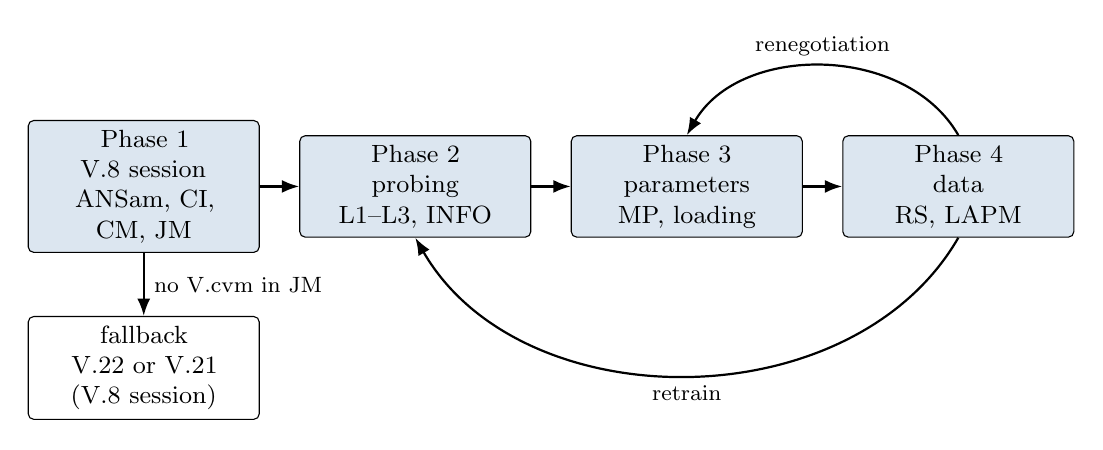
\begin{tikzpicture}[x=1cm,y=1cm,font=\small,
  ph/.style={draw,rounded corners=2pt,fill=ituhead,minimum height=0.9cm,
    text width=2.7cm,align=center},
  arr/.style={-{Latex[length=2.2mm]},thick}]
\node[ph] (p1) {Phase 1\\V.8 session\\ANSam, CI, CM, JM};
\node[ph,right=0.5cm of p1] (p2) {Phase 2\\probing\\L1--L3, INFO};
\node[ph,right=0.5cm of p2] (p3) {Phase 3\\parameters\\MP, loading};
\node[ph,right=0.5cm of p3] (p4) {Phase 4\\data\\RS, LAPM};
\draw[arr] (p1) -- (p2); \draw[arr] (p2) -- (p3); \draw[arr] (p3) -- (p4);
\node[ph,below=0.8cm of p1,fill=white] (fb) {fallback\\V.22 or V.21\\(V.8 session)};
\draw[arr] (p1.south) -- (fb.north) node[midway,right,font=\footnotesize] {no \recname{} in JM};
\draw[arr] (p4.north) to[out=120,in=60] node[above,font=\footnotesize] {renegotiation} (p3.north);
\draw[arr] (p4.south) to[out=-120,in=-60] node[below,font=\footnotesize] {retrain} (p2.south);
\end{tikzpicture}
\caption{The phases of a call}
\label{fig:phases}
\end{figure}

\section{Reference configuration and interfaces}\label{sec:ref}
\subsection{Reference configuration}
Figure~\ref{fig:refconf} gives the reference configuration.  Reference
point~P is the signal interface: the DCE gives its transmitted signal to
the terminal as linear PCM samples and takes the received signal from it
in the same form.  The terminal is whatever carries the speech path: a
UE, an IMS client, a gateway between the IMS and another network, or a
circuit-switched mobile terminal.  Everything from one reference point P
to the other is the speech path.

\begin{figure}[htbp]
\centering
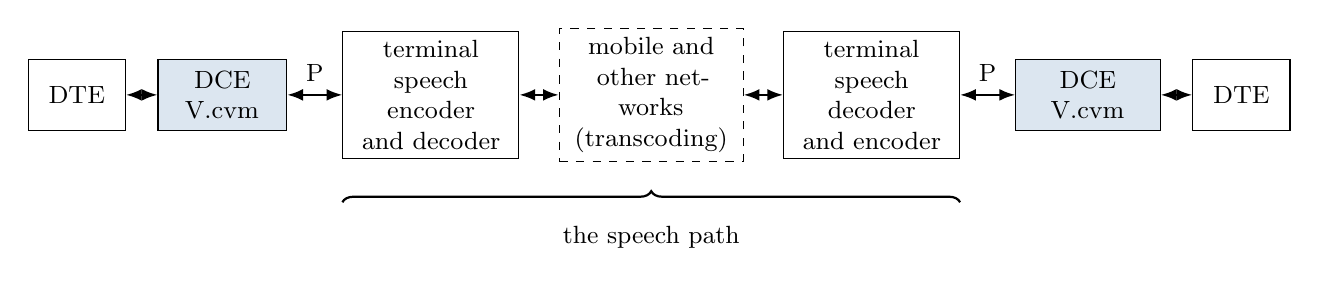
\begin{tikzpicture}[x=1cm,y=1cm,font=\small,
  box/.style={draw,minimum height=0.9cm,align=center},
  arr/.style={{Latex[length=2mm]}-{Latex[length=2mm]},thick}]
\node[box,text width=1.0cm] (dte1) {DTE};
\node[box,text width=1.4cm,right=0.4cm of dte1,fill=ituhead] (dce1) {DCE\\\recname};
\node[box,text width=2.0cm,right=0.7cm of dce1] (t1) {terminal\\speech encoder\\and decoder};
\node[box,text width=2.1cm,right=0.5cm of t1,dashed] (net) {mobile and\\other networks\\(transcoding)};
\node[box,text width=2.0cm,right=0.5cm of net] (t2) {terminal\\speech decoder\\and encoder};
\node[box,text width=1.6cm,right=0.7cm of t2,fill=ituhead] (dce2) {DCE\\\recname};
\node[box,text width=1.0cm,right=0.4cm of dce2] (dte2) {DTE};
\draw[arr] (dte1) -- (dce1); \draw[arr] (dce1) -- (t1) node[midway,above=1pt] {P};
\draw[arr] (t1) -- (net); \draw[arr] (net) -- (t2);
\draw[arr] (t2) -- (dce2) node[midway,above=1pt] {P}; \draw[arr] (dce2) -- (dte2);
\draw[decorate,decoration={brace,amplitude=4pt},thick]
  ([yshift=-0.55cm]t1.south west) -- ([yshift=-0.55cm]t2.south east)
  node[midway,below=5pt] {the speech path};
\end{tikzpicture}
\caption{Reference configuration}
\label{fig:refconf}
\end{figure}

\subsection{The signal interface (reference point P)}\label{sec:pointp}
At reference point P:
\begin{enumerate}[label=\alph*)]
\item samples shall be 16~bit linear PCM, two's complement, at 8000~Hz
  (narrowband operation) or 16000~Hz (wideband operation).  A DCE shall
  support 8000~Hz and may support 16000~Hz.  The rate is the terminal's;
  the DCE learns the band the path carries by probing, not from the rate.
\item the DCE's transmitted signal shall not exceed $-9$~dBFS rms in
  any 20~ms frame and should be at $-12 \pm 2$~dBFS in the comb modes
  and $-15 \pm 2$~dBFS in the parametric mode (whose pulse train has a
  peak factor of 13~dB, clause~\ref{sec:parametric}), so that no
  terminal gain stage limits it and the codec's gain quantizers are in
  their range.  The received level is whatever the path delivers;
  the DCE shall accept $-30$ to $-3$~dBFS.
\item the terminal should pass the samples to and from the speech codec
  without acoustic processing (echo cancellation, noise suppression,
  automatic gain control, voice activity detection with comfort noise)
  between P and the codec.  Where the terminal cannot disable them, the
  DCE shall still operate, with the modes the probing finds usable.
\item the sample clocks of the two terminals are independent.  The DCE
  shall tolerate a difference of $\pm 200$~ppm between its transmit clock
  and the received signal's, and the steps of clause~\ref{sec:timing}.
\end{enumerate}

\itunote{A DCE in a UE must reach the speech codec's PCM interface.  The
acoustic path (loudspeaker to microphone) is not a signal interface of
this Recommendation.}

\subsection{Interchange circuits}
The DTE interface is the serial asynchronous interface of \rec{V.250}
(clause~\ref{sec:dte}), on any physical interface a V.250 DCE may have.

% ---------------------------------------------------------------- startup
\section{Start-up procedures}\label{sec:startup}
\subsection{General}
A DCE of this Recommendation shall perform the start-up procedures of
\rec{V.8}: the answering DCE transmits ANSam; the calling DCE transmits CI
and, on detecting ANSam, CM; the answering DCE answers with JM; the
calling DCE acknowledges with CJ.  The V.21 modulation of CI, CM, JM and
CJ passes through every mode of the codecs
(Appendix~\ref{app:measurements}, Table~\ref{tab:modsurvive}), and ANSam's
2100~Hz tone, with its phase reversals, disables the network's echo
cancellers (as it is meant to), which matters at a gateway to the PSTN.

\subsection{Capability indication}
The calling DCE shall indicate its support of this Recommendation in CM
and the answering DCE in JM, as Annex~\ref{annex:v8} specifies, together
with the modulation modes of its fallback (V.22 and V.21) and the
protocol (LAPM).  The indication carries:
\begin{itemize}
\item the version of this Recommendation (1);
\item the signal interface rate: 8000, or 16000~Hz;
\item the modes of clause~\ref{sec:modulation} the DCE supports;
\item whether the DCE can carry facsimile (Annex~\ref{annex:fax}).
\end{itemize}

\subsection{Outcome}
When both CM and JM carry the indication, both DCEs proceed to the
probing of clause~\ref{sec:probing} on the completion of the V.8
procedures (CJ sent, or JM ended), within the time \rec{V.8} allows for the
start of the selected modulation.  Otherwise the DCEs proceed to the
common modulation mode of highest rate among those indicated, V.22 then
V.21, as \rec{V.8} and that Recommendation specify, and this Recommendation
has nothing more to say about the call.

An answering DCE that has agreed on this Recommendation and detects the
end of CM (30~ms of the line 30~dB below CM's level) without having
decoded CJ shall take the end of CM for CJ: a codec at a low mode can
garble CJ's three zero octets, and the calling DCE's INFO0 follows CJ by
only 175~ms.

\itunote{A legacy V series DCE on the PSTN, reached through a gateway,
indicates its own modulation modes (V.34, V.32bis, ...) and none of this
Recommendation's.  Of its modulation modes, V.22 is the fastest the
codec carries (Table~\ref{tab:modsurvive}): a DCE of this Recommendation
should not indicate modulation modes above V.22 in CM when it knows the
speech path to be a codec's, so that the legacy DCE selects V.22 at once
rather than fail at V.34 and renegotiate.}

\subsection{Timing}
The DCEs' timers for the V.8 procedures are \rec{V.8}'s.  The probing of
clause~\ref{sec:probing} shall begin within 200~ms of the end of the V.8
procedures and shall be complete, with the first data symbols sent,
within 21~s (each direction's INFO0, L1, L2, L3 and INFO1 take about 7~s
with the messages at 200~bit/s, and the MP exchange 1 to 4~s; the
start-up takes 15 to 21~s); a DCE that has not received its peer's
INFO0 within 6~s of the end of the V.8 procedures shall fall back to
V.22 by restarting the V.8 procedures, once.

% ---------------------------------------------------------------- probing
\section{Probing and mode selection}\label{sec:probing}
\subsection{Purpose}
Probing measures the speech path as the signal set will see it:
\begin{enumerate}[label=\alph*)]
\item the band carried, from which the signal interface rate of the far
  end and the codec's bandwidth mode follow;
\item the noise per tone against a multitone signal of the signal set's
  own form, from which the loading follows;
\item the round-trip delay, for the timers of the link layer.
\end{enumerate}
Each direction is probed and loaded separately: the two directions of a
mobile call go through different codecs, radio links and jitter buffers.

\subsection{Phase 2: the probing signals}\label{sec:phase2}
After the V.8 procedures each DCE transmits, in turn as
Figure~\ref{fig:probing} shows:
\begin{enumerate}
\item \textbf{INFO0}: its signal interface rate, the modes it supports and
  the comb it will probe with, modulated as clause~\ref{sec:infomod}
  specifies;
\item \textbf{L1}: the probing combs of Annex~\ref{annex:probe}: each
  comb the DCE supports for the band of its signal interface, in turn
  (200, 300 and 400~Hz spacing, Table~\ref{tab:combs}), all tones loaded,
  each tone with a differential phase sequence known to both, 0.6~s a
  comb;
\item \textbf{L2}: the 200~Hz comb with the 22.5~ms symbol, for 0.5~s, so
  that the receiver may compare the two symbol periods;
\item \textbf{L3}, where the DCE indicated the parametric mode: that
  mode's probing signal of Annex~\ref{annex:probe}, 40 symbols of P20
  and 80 of P10 with lags known to both, each part with its preamble;
\item \textbf{INFO1}: what it measured of its peer's L1 to L3 as the
  loading it asks for (clause~\ref{sec:loading}), and its own round-trip
  estimate.
\end{enumerate}
Each part follows the last after 100~ms of silence.  The calling DCE
transmits its INFO0, L1, L2 and L3 first; the answering DCE begins its
INFO0 50~ms after the end of the calling DCE's L3 and transmits INFO0, L1,
L2, L3 and its INFO1; the calling DCE then transmits its INFO1 50~ms after
the end of the answering DCE's.  The calling DCE's INFO1 cannot carry what
it measured before it has received anything, which is why it comes last.
A DCE that misses its peer's INFO1 takes the loading from the peer's
first MP (clause~\ref{sec:phase3}), which has INFO1's layout.  The
probing signal's level is $-12$~dBFS.

\begin{figure}[htbp]
\centering
\resizebox{\textwidth}{!}{%
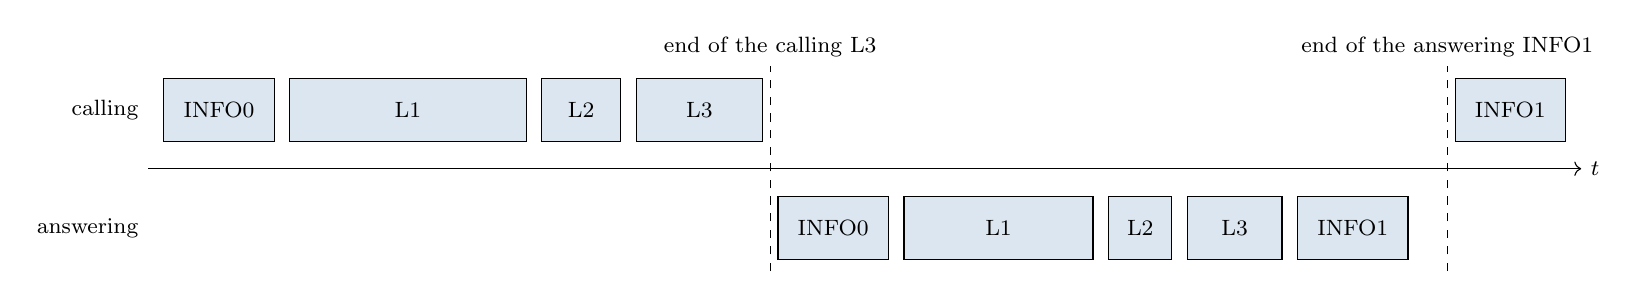
\begin{tikzpicture}[x=1cm,y=1cm,font=\footnotesize]
\draw[->] (0,0) -- (18.2,0) node[right] {$t$};
\node[left] at (0,0.75) {calling};
\node[left] at (0,-0.75) {answering};
\foreach \x/\w/\n in {0.2/1.4/INFO0,1.8/3.0/L1,5.0/1.0/L2,6.2/1.6/L3,16.6/1.4/INFO1} {
  \draw[fill=ituhead] (\x,0.35) rectangle ++(\w,0.8) node[midway] {\n};}
\foreach \x/\w/\n in {8.0/1.4/INFO0,9.6/2.4/L1,12.2/0.8/L2,13.2/1.2/L3,14.6/1.4/INFO1} {
  \draw[fill=ituhead] (\x,-1.15) rectangle ++(\w,0.8) node[midway] {\n};}
\draw[dashed] (7.9,-1.3) -- (7.9,1.3);
\node[above] at (7.9,1.3) {end of the calling L3};
\draw[dashed] (16.5,-1.3) -- (16.5,1.3);
\node[above] at (16.5,1.3) {end of the answering INFO1};
\end{tikzpicture}}
\caption{Phase 2: the probing signals (durations not to scale)}
\label{fig:probing}
\end{figure}

\subsection{Modulation of the INFO and MP messages: the message mode}\label{sec:infomod}
INFO0, INFO1 and the MP messages of clause~\ref{sec:phase3} shall be
transmitted in the \emph{message mode}, which is:
\begin{enumerate}[label=\alph*)]
\item where both DCEs indicated the parametric mode in CM and JM
  (Annex~\ref{annex:v8}), the parametric mode with the 20~ms symbol
  (P20, clause~\ref{sec:parametric}): the preamble of that clause, then
  the message's bits four to a lag symbol as clause~\ref{sec:mapping}
  maps them, unscrambled, padded with flags to whole symbols;
\item otherwise the \emph{robust mode} of clause~\ref{sec:modes}: the FSK
  of \rec{V.21} at 300~bit/s, channel~1 from the calling DCE and
  channel~2 from the answering DCE as \rec{V.8} uses them for CM and JM.
\end{enumerate}
A message is an HDLC frame (flags, FCS) of \rec{V.42} with the message's
octets as the information field.  Each message is sent twice; the
receiver takes the first copy whose FCS checks.  V.21's bit error ratio
was measured below $10^{-2}$ through every mode of AMR but 4.75~\kbs{},
of AMR-WB but 6.6, and of EVS but 9.6 wideband
(Appendix~\ref{app:measurements}, Table~\ref{tab:fsk}); the parametric
mode's lag symbol error ratio was zero through all of them but AMR 4.75
(Table~\ref{tab:pitch}), which is why it carries the messages where both
DCEs have it.  Measured end to end, through a receiver of two filters matched
over the bit with its own bit clock (Appendix~\ref{app:impl}), V.21's bit
error ratio was 1 to $3 \cdot 10^{-2}$ at AMR 5.15 to
6.7~\kbs{}: messages in V.21 are surest from AMR 7.4~\kbs{} up.  A
receiver may retry a P20 message whose FCS fails with the second most
likely lag on the few least reliable symbols.

\itunote{V.34 modulates INFO and MP at 600~bit/s with differential phase
modulation on two tones.  Through AMR at 7.4~\kbs{} and below no
differential phase modulation measured kept a symbol error ratio below
$10^{-1}$, while 300~bit/s FSK did (Table~\ref{tab:fsk}); so this
Recommendation sends its messages as V.8 sends CM and JM, or on the
codec's pitch lag, which is surer still.}

\subsection{The loading}\label{sec:loading}
From its peer's L1 and L2 the receiving DCE shall estimate, for each tone
of the comb and each of the two symbol periods, the root mean square
phase error of the received tone symbols against the known sequence, and
for each tone the mean received level and the rms change of its
magnitude from one symbol to the next (in dB).  It shall then choose:
\begin{enumerate}[label=\alph*)]
\item the band: the tones whose level is within 20~dB of the strongest
  tone's; tones outside are not loaded (this finds the codec's band);
\item the comb and the symbol period: those giving the greatest number
  of bits per second over the tones loaded by c); a comb of fewer tones,
  more widely spaced, wins where the codec's noise against each tone of a
  denser comb is too high (Appendix~\ref{app:measurements});
\item the modulation order of each tone, from its phase error $\sigma$:
  DQPSK where $\sigma \le 20^\circ$, 8-DPSK where $\sigma \le 9^\circ$ and
  the mode set allows it, none where $\sigma > 20^\circ$; and on a loaded
  tone, from the rms change $\sigma_A$ of its magnitude from one symbol of
  L1 to the next, two amplitude rings where $\sigma_A \le 0.8$~dB and four
  where $\sigma_A \le 0.4$~dB, where both DCEs have the amplitude loading
  of clause~\ref{sec:qam} and the mode set allows it;
\item the code rate of the Reed-Solomon code (Annex~\ref{annex:rs}) from
  the measured tone symbol error ratio over the loaded tones: rate~7/8
  below $10^{-3}$, 3/4 below $10^{-2}$, 1/2 otherwise (in the parametric
  mode, from the lag symbol error ratio of L3 the same way);
\item the mode: the comb of b) where it loads four tones or more and
  carries more after the code of d) than the parametric mode would;
  otherwise the parametric mode (clause~\ref{sec:parametric}), with the
  10~ms symbol where no lag symbol of L3's P10 part was in error, else
  the 20~ms symbol where at most one of its P20 part's 40 symbols was (at
  the code rate 1/2 where one was); else no data mode:
  the DCE asks in MP for no loading (Annex~\ref{annex:probe}) and both
  DCEs wait in the message mode, retraining as clause~\ref{sec:reneg}
  says, until the codec's mode carries one (AMR at 4.75~\kbs{} is the
  one codec mode measured that carries none; a network leaves a call
  there only at the worst coverage).
\end{enumerate}
The thresholds in c) give a tone symbol error ratio of about $10^{-2}$
at the threshold for Gaussian phase error, which the code of
Annex~\ref{annex:rs} corrects to below $10^{-6}$ at rate~3/4.  The
loading is sent to the peer in INFO1 and MP as a bitmap of the comb with
two bits a tone (none, DQPSK, 8-DPSK), with a second such bitmap for the
amplitude rings where any tone has them (Annex~\ref{annex:probe}), or as
the parametric mode and its symbol period.

\subsection{Phase 3: parameter exchange}\label{sec:phase3}
Each DCE transmits an \textbf{MP} message with the loading it asks for in
the direction it receives, the symbol period and the code rate, in the
manner of \rec{V.34}'s MP sequence; it shall
transmit MP until it has received its peer's MP with the acknowledgement
bit set, then once more with its own acknowledgement bit set, and begin
data transmission (phase~4) with the loading its peer asked for.  Both
directions enter phase~4 within 100~ms of each other.

\subsection{Renegotiation and retrain}\label{sec:reneg}
During phase~4, a DCE whose receiver measures a phase error or an error
ratio over the thresholds of clause~\ref{sec:loading} on tones it loaded,
or well under them on tones it did not load, should ask for a
\emph{renegotiation}: it sends the control sequence of
clause~\ref{sec:control} and the DCEs exchange MP messages in the
message mode (clause~\ref{sec:infomod}) with the new loading, then
resume data; the code's interleaver is flushed and restarted.  A DCE
that loses the symbol timing, or the signal, or decodes no codeword for
2~s (or 2.5 interleaver blocks where that is longer) shall ask for a
\emph{retrain}: the control sequence, then MP messages with the retrain
bit set (Table~\ref{tab:loading}); after the exchange both DCEs return to
phase~2, the calling DCE's INFO0 3~s after it (so that the answering
DCE's last MP is through).  The
codec's mode changes with the radio conditions, and the loading shall
follow it; a renegotiation shall take no more than 500~ms and a DCE
shall not refuse one.

A DCE whose receive direction is in the parametric mode, or in no data
mode (clause~\ref{sec:loading}~e)), has nothing that measures the combs:
it should ask for a retrain 30~s after entering that state and every
60~s while it lasts, so that a codec mode that has improved is found and
used.  In the parametric mode it shall keep $\bar c$, the mean over the
last 2~s of the decided lags' normalized autocorrelation $c$
(clause~\ref{sec:parametric}).  While $\bar c$ is below 0.85 it need not
ask for those retrains: no codec mode measured that gives $\bar c$ below
0.85 carries a comb.  When $\bar c$ rises to 0.85 or more from below, it
should ask for a retrain at once rather than at the next 60~s, though not
in the first 30~s of phase~4.  The threshold has 0.02 of hysteresis:
$\bar c$ is below it once under 0.83 and rises through it at 0.87, so
that $\bar c$ wavering about 0.85 does not retrain again and again.  At or
above 0.85 the periodic retrains stay: $\bar c$ there does not say
whether a comb would pass.

\itunote{$\bar c$ does not order the codec modes by what they carry, so it
cannot replace the retrain (Appendix~\ref{app:measurements},
Table~\ref{tab:pquality}).  Every mode measured in which a comb loads
four tones or more gave $\bar c$ of 0.875 or more (AMR 10.2 the least),
but modes in which none does gave as much as 0.938 (EVS 9.6) and 0.920
(AMR 7.95 loads five): the long-term predictor of a codec at a low mode
may code the pulse train's period better than one at a higher mode that
spends its bits on the excitation.  Below 0.85 are only the lowest modes
(AMR 4.75 to 5.9, AMR-WB 6.6, EVS 7.2 and 8.0), none of which carries a
comb, and $\bar c$ over 2~s varies by at most 0.075 there; so $\bar c$
saves the retrains where they cannot succeed, and its rise through 0.85,
a codec mode leaving that range, is the earliest sign one may.}

% ---------------------------------------------------------------- modulation
\section{Modulation}\label{sec:modulation}
% modulation.tex - clause 10 of v_cvm.tex: the signal set
\subsection{Signal set}\label{sec:modes}
The signal set has three modes, Table~\ref{tab:modes}.  A DCE shall
support the robust mode and the narrowband mode; it may support the
wideband mode (which needs the signal interface at 16000~Hz).

\begin{table}[htbp]
\caption{The modes of the signal set}
\label{tab:modes}
\small
\begin{tabularx}{\textwidth}{>{\raggedright\arraybackslash}p{2.3cm}>{\raggedright\arraybackslash}X>{\raggedright\arraybackslash}X>{\raggedright\arraybackslash}X}
\toprule
\rowcolor{ituhead}\thd{} & \thd{Robust (R)} & \thd{Narrowband (N)} & \thd{Wideband (W)} \\
\midrule
Signal & the FSK of \rec{V.21}: channel~1 (980/1180~Hz) from the calling DCE, channel~2 (1650/1850~Hz) from the answering DCE, 300~bit/s & a comb of tones at 200, 300 or 400~Hz spacing in the band 300 to 3400~Hz (16, 11 or 8 tones), DPSK & a comb of tones at 200, 300 or 400~Hz spacing in the band 300 to 6900~Hz (33, 23 or 17 tones), DPSK \\
Symbol & 3.33~ms (one bit) & 20~ms (a codec frame): a useful part of whole cycles of the spacing and a cyclic prefix (clause~\ref{sec:timing}); the 200~Hz comb also 22.5~ms & as N \\
Modulation & binary FSK & DQPSK, or 8-DPSK on tones with a low enough phase error & as N \\
Raw rate & 300~bit/s & 1600~bit/s (16 tones at 200~Hz, DQPSK, 20~ms), 1100 (11 at 300~Hz), 800 (8 at 400~Hz); half as much again with 8-DPSK & 3300~bit/s (33 tones at 200~Hz, DQPSK, 20~ms), 2300 (23 at 300~Hz), 1700 (17 at 400~Hz); half as much again with 8-DPSK \\
Use & INFO and MP messages, control sequences; data through codecs that carry nothing else & data & data \\
Passes (measured) & every AMR mode but 4.75, every AMR-WB mode but 6.6, every EVS mode but 9.6 wideband & AMR 12.2 (every comb), AMR 10.2 and two AMR 12.2 codecs in tandem (the 300 and 400~Hz combs), AMR-WB from 12.65, EVS 13.2 (N400) and 24.4 (every comb, 8-DPSK) & AMR-WB 23.85 (28 tones of W200), 15.85 (16 of W300), 12.65 (7 of W300); EVS 24.4 (W300), 48 and above (every comb, 8-DPSK); the super wideband combs through EVS at 48~\kbs{} and above \\
\bottomrule
\end{tabularx}
\end{table}

\itunote{The modes were chosen from measurements (Appendix~\ref{app:measurements}).
Through AMR at 7.4~\kbs{} and below, no differential phase modulation
measured kept a symbol error ratio below $10^{-1}$, on one carrier or many;
only 300~bit/s FSK did.  Through AMR at 12.2 and AMR-WB at 23.85~\kbs{},
a comb of 16 tones at 200~Hz spacing with DQPSK and a symbol of 20 to
22.5~ms kept its tone symbol error ratio at or below $10^{-2}$; combs of
32 tones at 100~Hz spacing did not (the codec's noise against each tone
grows faster than the number of tones), and 8-DPSK held only on the
better tones.  Fewer tones, more widely spaced, keep working where more
do not: through AMR at 10.2~\kbs{} and through two AMR codecs in tandem
the 11-tone comb at 300~Hz spacing kept $3 \cdot 10^{-3}$ while the
16-tone comb went to $3 \cdot 10^{-2}$, and through AMR-WB at 15.85 the
300~Hz comb loads 16 tones where the 200~Hz comb loads 10; so the signal
set has three combs for each band and the probing chooses.  A single
carrier at 600~baud (V.22's) passes AMR~12.2 as
well, at 1200~bit/s; the comb carries a third more at the same symbol
error ratio and loads itself to the codec.}

\subsection{The comb}\label{sec:comb}
The comb's tones are at the frequencies
\[ f_k = k \cdot \Delta f, \qquad k = k_{\min}, \ldots, k_{\max}, \]
as Table~\ref{tab:combs} gives them.
\begin{table}[htbp]
\caption{The combs}
\label{tab:combs}
\small
\begin{tabular}{llcccccc}
\toprule
\rowcolor{ituhead}\thd{Code} & \thd{Comb} & $\Delta f$ (Hz) & $k$ & \thd{Tones} & \thd{Band (Hz)} & $T_u$ (ms) & $T_g$ (ms) \\
\midrule
0 & N200 & 200 & 2--17 & 16 & 400--3400 & 15 (or 20) & 5 (or 2.5) \\
1 & N300 & 300 & 1--11 & 11 & 300--3300 & 10 & 10 \\
2 & N400 & 400 & 1--8 & 8 & 400--3200 & 15 & 5 \\
3 & W200 & 200 & 2--34 & 33 & 400--6800 & 15 & 5 \\
4 & W300 & 300 & 1--23 & 23 & 300--6900 & 10 & 10 \\
5 & W400 & 400 & 1--17 & 17 & 400--6800 & 15 & 5 \\
6 & S200 & 200 & 2--69 & 68 & 400--13800 & 15 & 5 \\
7 & S300 & 300 & 1--46 & 46 & 300--13800 & 10 & 10 \\
8 & S400 & 400 & 1--35 & 35 & 400--14000 & 15 & 5 \\
9--15 & -- & \multicolumn{6}{l}{reserved} \\
\bottomrule
\end{tabular}
\end{table}
The narrowband combs N200, N300 and N400 are for the signal interface
at 8000~Hz, the wideband combs W200, W300 and W400 for 16000~Hz, and the
super wideband combs S200, S300 and S400 for 32000~Hz (for the EVS
codec's super wideband modes, Appendix~\ref{app:evs}).  The probing (clause~\ref{sec:probing}) decides which
tones are loaded; the transmitter sends nothing on a tone that is not.
The transmitted signal in the useful part of symbol $n$ is
\[ s_n(t) = A \sum_{k \in \mathcal{L}} \cos\bigl(2\pi f_k t + \varphi_{n,k}\bigr), \qquad 0 \le t < T_u, \]
where $\mathcal{L}$ is the set of loaded tones, $\varphi_{n,k}$ the tone's
phase in this symbol and $A$ the amplitude that gives the level of
clause~\ref{sec:pointp}~b) over the loaded tones.  The useful period $T_u$
is a whole number of cycles of $\Delta f$, so that the tones are
orthogonal over it.

\subsection{Symbol timing and the cyclic prefix}\label{sec:timing}
A symbol consists of a cyclic prefix of $T_g$ followed by the useful part
of $T_u$: the prefix is the last $T_g$ of the useful part, transmitted
first, so that the signal is continuous across each symbol except for the
phase steps at the symbol's start.  The symbol periods are
\begin{itemize}
\item \textbf{20~ms}, the period of a codec frame, for every comb: $T_u$
  and $T_g$ as Table~\ref{tab:combs} gives them (three cycles of the
  spacing for the 200 and 300~Hz combs, six for the 400~Hz combs), so
  that one symbol's phase steps fall in each frame and the prefix spans
  the codec's transient after them (a subframe of 5~ms, or two for the
  300~Hz combs);
\item \textbf{22.5~ms}, for the N200 comb only: $T_u = 20$~ms (four
  cycles), $T_g = 2.5$~ms, for codecs that gain from the longer integration
  (the probing compares the two).
\end{itemize}
The receiver shall integrate each tone over the useful part only.  A
receiver shall acquire the symbol timing from the cyclic prefix (the
correlation of the signal with itself $T_u$ earlier peaks over the prefix)
and shall re-acquire it within two symbols after a step of the received
timing of up to $\pm 20$~ms, which a jitter buffer's adaptation causes
(Appendix~\ref{app:terminal}).  Differential modulation makes the symbol
after such a step the only one lost.

\subsection{The codec frame and the symbol}\label{sec:align}
The symbols are not aligned to the codec's frames, and no alignment is
signalled: the position of the symbols' phase steps within the frame was
found to make no difference to the tone symbol error ratio
(Appendix~\ref{app:measurements}, Table~\ref{tab:combnb}: the 20~ms
symbol at a frame boundary and 10~ms off it), which the codec's 5~ms
subframes and its long-term predictor explain: the step is coded in the
subframe it falls in, wherever that is.  The 20~ms symbol is chosen for
its rate (12 per cent more than the 22.5~ms symbol) and for its match
with the frame erasures: one erased frame is one symbol.

\subsection{Differential phase modulation}
Each loaded tone carries, per symbol, the phase difference
$\varphi_{n,k} - \varphi_{n-1,k}$, one of four values for DQPSK or eight for
8-DPSK, mapped from the bits as Table~\ref{tab:gray} shows.  The first
symbol of phase~4, and the first after a renegotiation, carries no data:
it is the phase reference.  The receiver decides each tone symbol from the
difference of the tone's phases in two consecutive symbols; no carrier
recovery and no equalization are required, and a frequency offset between
the DCEs' clocks of $\Delta f_c$ appears as a constant phase rotation of
$2\pi \Delta f_c T$ per symbol, which the receiver should estimate from
the decisions and remove.

\subsection{Loading and raw rate}
The raw rate is
\[ R = \frac{1}{T_u + T_g} \sum_{k \in \mathcal{L}} b_k, \]
with $b_k = 2$ for a DQPSK tone and 3 for an 8-DPSK tone: 1600~bit/s for the
16 DQPSK tones of N200 at the 20~ms symbol, 1100 for N300, 800 for N400,
3300 for W200, and half as much again with 8-DPSK on all tones.  The loading of clause~\ref{sec:loading} chooses $\mathcal{L}$
and the $b_k$; a loading with fewer than 4 tones shall not be used (the
DCE renegotiates or retrains).

\subsection{Control sequences during data}\label{sec:control}
A DCE that wishes to renegotiate (clause~\ref{sec:reneg}) shall send, in
place of data, the control sequence: eight consecutive symbols with the
phase difference $180^\circ$ on every loaded tone, then its MP in the
robust mode.  A receiver that decodes four such symbols in a row shall
stop delivering data to the inner decoder, flush, answer with the same
sequence if it has not sent one, and proceed to the MP exchange.  The
sequence cannot occur in scrambled data for more than two symbols with a
probability above $10^{-9}$ on 8 tones.

\subsection{Scrambling}
The bits given to the mapping of clause~\ref{sec:mapping} shall be
scrambled with the generating polynomials of \rec{V.34}: $1 + x^{-18} + x^{-23}$
in the calling DCE's transmitter and $1 + x^{-5} + x^{-23}$ in the
answering DCE's (GPC and GPA), self-synchronizing as in that
Recommendation.  The scrambler is reset at the start of phase~4 and after
each renegotiation.

\subsection{Quick start}\label{sec:quick}
A DCE may keep, for the last number dialled or answered, the loading and
the symbol period of the last call, and offer them in INFO0 as the mode
to start with.  If its peer accepts in its INFO0, phase~2 is reduced to L1 of
0.5~s for a check of the loading, and the DCEs proceed to phase~3; this
is in the manner of \rec{V.92}'s quick connect.  A loading so offered
shall still be checked by the receiver against the thresholds of
clause~\ref{sec:loading}.

\subsection{Loading with amplitude: for further study}\label{sec:qam}
The MP message carries a loading value reserved for QAM constellations of
16 and 64~points per tone, with the 16-state four-dimensional trellis code
of \rec{V.34} across tone pairs as \rec{G.992.1} applies it.  Such a
loading is for the transform coding modes of the EVS codec, which carry
waveforms: through EVS at 48~\kbs{} and above a tone's amplitude was
measured to change by 0.3 to 1~dB rms from one symbol to the next, which
would hold two levels 6~dB apart (Appendix~\ref{app:evs}); through the
ACELP codecs it changes by 1.5 to 3~dB, and amplitude carries no bits.
The loading's parameters are for further study.  A DCE shall not
request it unless both DCEs have indicated the capability in CM and JM,
and shall fall back to DPSK when the peer does not confirm it in MP.


% ---------------------------------------------------------------- error
\section{Error control and framing}\label{sec:error}
\subsection{Structure}
The data of phase~4 pass, from the DTE towards the line, through:
\begin{enumerate}
\item \rec{V.42}: LAPM, with the V.42bis or V.44 compression the DCEs
  negotiate in XID (clause~\ref{sec:link});
\item the inner code: the Reed-Solomon code of Annex~\ref{annex:rs} over
  the HDLC frames' octets, as a continuous octet stream (the LAPM frames
  with their flags are the stream; no further framing is added);
\item the interleaver of Annex~\ref{annex:rs}, which spreads each
  codeword over several modulation symbols so that an erased codec frame
  costs each codeword a fraction of its symbols (its depth is 1 in the
  parametric mode);
\item the mapping of the coded bits onto the tone symbols, or the lag
  symbols of the parametric mode, of clause~\ref{sec:mapping}.
\end{enumerate}

\subsection{The code}
The inner code shall be the Reed-Solomon code over GF($2^8$) of
\rec{G.975} (the field of the primitive polynomial $x^8+x^4+x^3+x^2+1$,
the code generator of its clause on the RS(255,239) code), shortened to
the codeword lengths of Annex~\ref{annex:rs}: a codeword of $n$ octets
with $k$ information octets and $n-k = 2t$ check octets, correcting $t$
octets in error or $2t$ octets erased.  The code rates of
Table~\ref{tab:rates} are offered (Annex~\ref{annex:rs} shortens the
codewords to 32 octets, so that the interleaver's delay stays short).  A receiver should mark the octets of
an erased codec frame as erasures (clause~\ref{sec:erasure}).

\begin{table}[htbp]
\caption{Code rates of the inner code}
\label{tab:rates}
\small
\begin{tabular}{lccc}
\toprule
\rowcolor{ituhead}\thd{Rate} & \thd{Codeword $n$} & \thd{Information $k$} & \thd{Corrects $t$ octets / $2t$ erasures} \\
\midrule
7/8 & 32 & 28 & 2 / 4 \\
3/4 & 32 & 24 & 4 / 8 \\
1/2 & 32 & 16 & 8 / 16 \\
\bottomrule
\end{tabular}
\end{table}

\subsection{Erased frames}\label{sec:erasure}
A speech decoder conceals a lost or bad frame by extrapolating the
previous frame's parameters: the output over the erased frame keeps the
spectral envelope and the pitch of the signal before it and loses its
information.  A receiver of this Recommendation should detect an erased
frame -- from the phase errors of all its tones at once, or from the
tones' levels decaying together as concealment attenuates -- and mark the
tone symbols of the symbol or symbols it spans as erasures to the
Reed-Solomon decoder, which corrects twice as many erasures as errors.
With the interleaving depth of Annex~\ref{annex:rs} one erased 20~ms
frame erases one symbol in each of $D$ consecutive codewords' $D$
symbols, and is corrected at any code rate of Table~\ref{tab:rates};
frame erasure ratios of the mobile networks are below 2 per cent
(\tgpp{26.114}'s design targets), and the measured effect is in
Appendix~\ref{app:measurements}.  In the parametric mode the concealment
repeats the previous lag: the erased frame's symbol decodes as the
symbol before it, and the frame after it is often wrong as well (the
measured cost is two symbols an erasure, Table~\ref{tab:pitch}); the
receiver should detect the erasure from the level, which the concealment
attenuates, since the lag gives no sign of it.

\subsection{Mapping}\label{sec:mapping}
The interleaver's output bits shall be taken in order and mapped onto the
loaded tones of a symbol from the lowest tone to the highest, two bits to
a DQPSK tone and three to an 8-DPSK tone, Gray coded onto the phase
difference as Table~\ref{tab:gray} shows, and on a tone with amplitude
rings one or two bits more, onto its amplitude digit as
clause~\ref{sec:qam} says.  Bits left over at the end of a
symbol are carried into the next.  The receiver shall deliver, per tone
symbol, the hard decision and an indication of its reliability (the
distance of the received phase difference from the decision's, and of
the magnitude ratio from its decision boundary), so that
the Reed-Solomon decoder may be given erasures.  In the parametric mode
the bits are mapped four to a lag symbol, the first bit the most
significant, Gray coded onto the alphabet's index as Table~\ref{tab:lags}
shows; the receiver delivers the decision and its reliability as above.

\begin{table}[htbp]
\caption{Gray mapping of the phase difference}
\label{tab:gray}
\small
\begin{tabular}{lcccccccc}
\toprule
\rowcolor{ituhead}\thd{Phase difference} & 0 & 45 & 90 & 135 & 180 & 225 & 270 & 315 \\
\midrule
DQPSK bits & 00 & -- & 01 & -- & 11 & -- & 10 & -- \\
8-DPSK bits & 000 & 001 & 011 & 010 & 110 & 111 & 101 & 100 \\
\bottomrule
\end{tabular}
\end{table}

% ---------------------------------------------------------------- link
\section{Link layer, compression and DTE interface}\label{sec:dte}
\subsection{Link layer}\label{sec:link}
Above the inner code the DCEs shall operate \rec{V.42} LAPM.  The
detection phase of \rec{V.42} (ODP and ADP) is not needed and shall not be
used: both DCEs have indicated LAPM in the V.8 session; the originator
shall start LAPM's XID exchange on entering phase~4.  The DCEs should
negotiate \rec{V.44} compression, or \rec{V.42bis} where V.44 is not
available, in XID as those Recommendations specify.  LAPM's T401 shall be
set from the round-trip delay measured in phase~2 (clause~\ref{sec:phase2}),
with at least 1~s added for the interleaver's delay and the symbol
period, and 3~s in the parametric mode (a codeword takes 1.3~s at
200~bit/s); N401 should not exceed 64~octets at raw rates below
2400~bit/s, so that a frame fits in an interleaver block.

\itunote{The code of Annex~\ref{annex:rs} leaves LAPM an error ratio
below $10^{-6}$ in the loaded modes; LAPM is retained for the residual
errors, for the erased frames the code cannot cover, for flow control and
for compression.}

\subsection{DTE interface}
The DCE's DTE interface shall conform to \rec{V.250}, with:
\begin{enumerate}[label=\alph*)]
\item in \code{+MS} (modulation selection), the value \code{V\_CVM} for this
  Recommendation's modulation, with its automode fallback to V.22 and
  V.21 (\code{+MS=V\_CVM,1}); a DCE should make it its default on a speech
  path known to be a codec's.  \code{+MS?} reports the value, \code{+MS=?}
  includes it in the list.
\item the extended command \code{+CVM} (Table~\ref{tab:atcvm}) to constrain
  the mode set and to read the loading and the measurements of the
  current connection.
\item in the CONNECT result code, with \code{\textbackslash V1} or \code{X}
  settings that give the rate, the coded data signalling rate (clause~\ref{sec:conventions}) and the
  text \code{/CVM}; the raw rate is read with \code{+CVM?}.
\item the result code \code{+CVMR: <raw>,<coded>} (unsolicited, if enabled
  by \code{+CVM}) on each renegotiation.
\end{enumerate}

\begin{table}[htbp]
\caption{The +CVM command}
\label{tab:atcvm}
\small
\begin{tabularx}{\textwidth}{>{\raggedright\arraybackslash}p{6.0cm}X}
\toprule
\rowcolor{ituhead}\thd{Command} & \thd{Meaning} \\
\midrule
\code{+CVM=<modes>}\allowbreak\code{[,<rate>}\allowbreak\code{[,<report>]]} & \code{<modes>}: the modes allowed, a sum of 1 (robust), 2 (narrowband), 4 (wideband), 8 (8-DPSK permitted), 16 (the amplitude rings of clause~\ref{sec:qam} permitted), 32 (parametric); default all.  \code{<rate>}: the signal interface rate, 8000 or 16000.  \code{<report>}: 1 enables \code{+CVMR}. \\
\code{+CVM?} & \code{+CVM: <modes>,<rate>,<report>} and, while connected, a second line \code{+CVM: <raw tx>,<raw rx>,<coded tx>,<coded rx>,<symbol ms>,<tones tx>,<tones rx>,<code rate>,<renegotiations>,<erasures>} (the tones are 0 in the parametric mode). \\
\code{+CVM=?} & the ranges. \\
\bottomrule
\end{tabularx}
\end{table}

\subsection{S-registers}
S-register~44 (as a DCE of this Recommendation uses it) holds the number
of tones loaded in the receive direction of the last call, S-register~45
the number of renegotiations of the last call.  Both are read-only; the
loading kept for the quick start of clause~\ref{sec:quick} is the DCE's
own.

% ---------------------------------------------------------------- interworking
\section{Interworking}\label{sec:interworking}
\subsection{With V series DCEs on the PSTN}
A DCE of this Recommendation falls back to \rec{V.22} and \rec{V.21}
(clause~\ref{sec:startup}).  Through a gateway between the mobile network
and the PSTN the speech path has one codec (the mobile side's); V.22
passes AMR at 12.2~\kbs{} with its data intact and V.21 passes every
mode measured (Appendix~\ref{app:measurements}).  A gateway that detects
the V.8 session and switches its IP leg to \rec{G.711} or to the modem
relay of \rec{V.150.1} changes nothing for this Recommendation: the codec
that limits the path is the mobile side's.

\subsection{With DCEs of this Recommendation across two codecs}
A mobile-to-mobile call, or a call through a transcoding gateway, has two
or more codecs in tandem in each direction.  The probing of
clause~\ref{sec:probing} measures the tandem as one channel; the loading
follows the measurement.  The throughput through two codecs is lower than
through one (Appendix~\ref{app:measurements} gives the measured figures
for AMR after AMR), and the retrain timers allow for the longer delay.

\subsection{With facsimile}
Facsimile terminals are served through Annex~\ref{annex:fax}: the DCE
terminates the \rec{T.30} session on its side and carries it as \rec{T.38}
packets in the data link.  The modulations of a facsimile terminal
(V.27ter, V.29, V.17) do not pass the codecs (Table~\ref{tab:modsurvive}).

% ---------------------------------------------------------------- performance
\section{Performance}\label{sec:performance}
A DCE of this Recommendation shall meet the following, measured through
the reference codecs of Appendix~\ref{app:measurements} with no frame
erasures and the signal interface at 8000~Hz, with the method of that
appendix:
\begin{enumerate}[label=\alph*)]
\item through AMR at 12.2~\kbs{} it shall connect in a narrowband mode
  with a raw rate of at least 1200~bit/s in each direction, and with the
  Reed-Solomon code at rate~3/4 or better;
\item through AMR at 7.95 and 7.4~\kbs{} and AMR-WB at 6.6~\kbs{} it
  shall connect in the parametric mode with a raw rate of at least
  200~bit/s in each direction, and through EVS at 9.6~\kbs{} narrowband
  of at least 400~bit/s (no mode of this Recommendation passes AMR at
  4.75~\kbs{}, whose radio conditions a network leaves only at the worst
  coverage: the DCEs wait in the message mode for a better codec mode);
\item through AMR-WB at 23.85~\kbs{} with the interface at 16000~Hz it
  shall connect in a wideband mode with a raw rate of at least
  2400~bit/s in each direction;
\item through EVS at 13.2~\kbs{} narrowband it shall connect in the
  narrowband mode (the N400 comb) with a raw rate of at least 800~bit/s;
  through EVS at 24.4~\kbs{} narrowband with a raw rate of at least
  2000~bit/s; through EVS at 48~\kbs{} wideband, with the interface at
  16000~Hz, of at least 4000~bit/s;
\item the error ratio delivered to LAPM shall be below $10^{-6}$ at the
  loading chosen by clause~\ref{sec:loading};
\item a frame erasure ratio of 1 per cent (independent erasures) shall
  not lower the coded rate in a comb mode by more than the code rate
  step of Table~\ref{tab:rates} (in the parametric mode an erasure costs
  two symbols, and the code rate~1/2 follows).
\end{enumerate}
The rates achievable are in Appendices~\ref{app:measurements} and
\ref{app:evs}.

% annexes.tex - the annexes of v_cvm.tex (normative)
\annex{Indication of this Recommendation's capabilities in V.8 and V.8bis}{v8}
\section{Encoding in CM and JM}
The CM and JM signals of \rec{V.8} are sequences of octets grouped in
categories (call function, modulation modes, protocols, GSTN access, PCM
modem availability, non-standard facilities).  This Recommendation needs
one bit of the modulation modes category to say ``\recname{} available'',
and an information field of two octets to say what of it.  The bit is an
allocation that ITU-T makes in a revision of \rec{V.8}; until it is made:
\begin{enumerate}[label=\alph*)]
\item the DCE shall send the information field of clause~\ref{sec:infofield}
  in the \emph{non-standard facilities} category of CM and JM, as \rec{V.8}
  provides for it, with the country code and the provider code of
  \rec{T.35} that the implementer holds, followed by the octets of
  Table~\ref{tab:infofield} with the identifier octet \code{0x43} (`C')
  first, so that a DCE of this Recommendation recognizes the field among
  a provider's other uses of the category;
\item the non-standard facilities category is the category octet
  \code{0x0F} followed by the NS field of \rec{V.8} (its length octet
  $K + L + M + 1$, the country code, the provider code's length $L$, the
  provider code, then the information: here the identifier and the two
  octets of the field), carried in extension octets of the form
  \code{xx010xxx}, five bits each, the field's bits from its first
  octet's least significant on, in bits 1 to 3 then 7 and 8 of each
  extension octet;
\item the DCE shall also set, in the modulation modes category, the bits
  of its fallback modulations (V.22 and V.21) and, in the protocols
  category, LAPM.
\end{enumerate}
On the allocation of the bit, a DCE shall set it and shall still send the
information field, in the category ITU-T assigns to it.

\section{The information field}\label{sec:infofield}
\begin{table}[htbp]
\caption{The information field}
\label{tab:infofield}
\small
\begin{tabularx}{\textwidth}{llX}
\toprule
\rowcolor{ituhead}\thd{Octet} & \thd{Bits} & \thd{Meaning} \\
\midrule
1 & 8--6 & version of this Recommendation: 001 \\
1 & 5 & signal interface at 16000~Hz (1), or 8000~Hz (0) \\
1 & 4 & facsimile of Annex~\ref{annex:fax} supported \\
1 & 3 & the amplitude loading of clause~\ref{sec:qam} supported \\
1 & 2 & the preset dictionary for \rec{V.44} of Annex~\ref{annex:v44dict} \\
1 & 1 & reserved, 0 \\
2 & 8 & robust mode (always 1) \\
2 & 7 & narrowband mode (always 1) \\
2 & 6 & wideband mode, 200~Hz comb \\
2 & 5 & wideband mode, 400~Hz comb \\
2 & 4 & 8-DPSK \\
2 & 3 & 22.5~ms symbol (the 20~ms symbol is always supported) \\
2 & 2 & quick start of clause~\ref{sec:quick} \\
2 & 1 & parametric mode (clause~\ref{sec:parametric}) \\
\bottomrule
\end{tabularx}
\end{table}
A DCE receiving an information field with a version it does not know
shall treat the peer as having version~1 and the capabilities the field's
bits it knows say.

\section{V.8bis}
A DCE that uses the procedures of \rec{V.8bis} shall carry the same
information field in the capabilities list of its MS and CL messages, in
the non-standard capability of that Recommendation, with the same
identifier octet.

\annex{The probing signals and the INFO messages}{probe}
\section{L1, L2 and L3}
L1 is each comb the transmitting DCE supports for the band of its
signal interface (Table~\ref{tab:combs}: N200, N300 and N400 at
8000~Hz; W200, W300 and W400 at 16000~Hz; S200, S300 and S400 at
32000~Hz), in the order of their codes, all tones loaded, DQPSK, with the
20~ms symbol, for 0.6~s each (30 symbols); L2 is the 200~Hz comb with the
22.5~ms symbol for 0.5~s (22 symbols).  The
phase difference transmitted on tone $k$ in symbol $n$ is given by two
bits taken from the scrambler of clause~\ref{sec:modulation} fed with
ones, started at the first symbol of L1 and run across the tones from the
lowest and across the symbols in order, so that the receiver, knowing
the sequence, measures the phase error of every tone symbol.  L1's first
symbol is the phase reference.  The level is $-12$~dBFS over all tones.

L3 is transmitted by a DCE that indicated the parametric mode
(clause~\ref{sec:parametric}): the P20 preamble and 40 symbols with the
20~ms symbol, then the P10 preamble and 80 symbols with the 10~ms
symbol, 1.84~s in all, the P10 part beginning where the P20 part ends
(the receiver takes the P10 part's timing from the P20 part's: the P10
preamble's lags are found poorly through AMR 10.2~\kbs{} and below); each symbol's index is four bits from the same
scrambler, continued from L2, so that the receiver, knowing the lags,
counts the symbols in error.  Its level is the parametric mode's,
$-15$~dBFS.

\section{What the receiver measures}
For each tone $k$ and each of L1 and L2 the receiver computes the root
mean square phase error $\sigma_k$ of the received phase differences
against the transmitted ones, after removing the mean (the clock offset's
rotation), the mean received level of the tone, the rms change
$\sigma_{A,k}$ of its magnitude from one symbol to the next in dB (for the
amplitude loading of clause~\ref{sec:qam}; L1's amplitude is constant),
and the fraction of tone symbols in error; for each part of L3, the
number of lag symbols in error.

\section{INFO0}
\begin{table}[htbp]
\caption{INFO0}
\small
\begin{tabularx}{\textwidth}{llX}
\toprule
\rowcolor{ituhead}\thd{Octet} & \thd{Bits} & \thd{Meaning} \\
\midrule
1 & 8--1 & the information field's octet 2 (Annex~\ref{annex:v8}): the modes supported \\
2 & 8--1 & the combs this DCE will probe with, a bit each for codes 0 to 7 of Table~\ref{tab:combs} (bit 8 for code 0) \\
3 & 8 & the same for code 8 \\
3 & 7 & quick start offered (the loading of octets 5 onwards is the last call's) \\
3 & 6 & quick start accepted (in the answering DCE's INFO0) \\
3 & 5 & the amplitude rings of clause~\ref{sec:qam} allowed (the DCE's \code{+CVM} permits them) \\
3 & 4--1 & reserved, 0 \\
4 & 8--1 & the DCE's transmit level in the data phases, in 0.5~dB below $-9$~dBFS \\
5-- & & with quick start: the loading of Table~\ref{tab:loading} \\
\bottomrule
\end{tabularx}
\end{table}

\section{INFO1 and MP}
\begin{table}[htbp]
\caption{INFO1 and MP: the loading asked for}
\label{tab:loading}
\small
\begin{tabularx}{\textwidth}{llX}
\toprule
\rowcolor{ituhead}\thd{Octet} & \thd{Bits} & \thd{Meaning} \\
\midrule
1 & 8 & MP only: acknowledgement (the peer's MP was received) \\
1 & 7--6 & symbol period: 00 20~ms, 01 22.5~ms, 10 10~ms (parametric mode only) \\
1 & 5--4 & code rate: 00 1/2, 01 3/4, 10 7/8 \\
1 & 3--1 & reserved, 0 \\
2 & 8 & MP only: retrain (both DCEs return to phase~2 after the exchange, clause~\ref{sec:reneg}) \\
2 & 7--1 & reserved, 0 \\
3 & 8--1 & round-trip delay this DCE measured, in 10~ms, 255 if unknown \\
4 & 8--5 & the comb: its code of Table~\ref{tab:combs}; 0 with the parametric mode \\
4 & 4 & the parametric mode (clause~\ref{sec:parametric}) is asked for, with the symbol period of octet~1: $N$ is then 0 \\
4 & 3 & amplitude rings: the second bitmap follows the first \\
4 & 2--1 & reserved, 0 \\
5 & 8--1 & number of tones $N$ in the comb, 8 to 68; 0 with the parametric mode, or when no data mode is asked for (clause~\ref{sec:loading}~e)) \\
6-- & & $N$ two-bit fields, the lowest tone first, packed from bit 8: 00 not loaded, 01 DQPSK, 10 8-DPSK, 11 reserved; where octet~4 bit~3 is set, $N$ more two-bit fields after them (from the next octet), the tones in the same order: 00 no rings, 01 two rings, 10 four rings (clause~\ref{sec:qam}), 11 reserved \\
\bottomrule
\end{tabularx}
\end{table}
Each message is an HDLC frame of \rec{V.42} (flags, the FCS of ISO/IEC
13239, no address or control octet) carrying the octets above, transmitted
twice in the message mode of clause~\ref{sec:infomod}; a receiver takes
the first copy whose FCS checks.  INFO0 is sent 100~ms after the end of
the V.8 procedures by the calling DCE; the answering DCE's INFO0 50~ms
after the end of the calling DCE's L3 (of L2 where there is no L3), and
its INFO1 100~ms after the end of its own L3; the calling DCE's INFO1
50~ms after the end of the answering DCE's.  Each DCE sends MP 100~ms
after the last INFO1, and after it has received its peer's MP with the
acknowledgement bit set, one more MP with its own set.

\annex{The inner code and its interleaver}{rs}
\section{The code}
The inner code is a Reed-Solomon code over GF($2^8$).  The field is
generated by the primitive polynomial $p(x) = x^8 + x^4 + x^3 + x^2 + 1$,
and the code generator polynomial is
\[ g(x) = \prod_{i=0}^{2t-1} (x - \alpha^i), \]
with $\alpha$ a root of $p(x)$: the field and the generator of the
RS(255,239) code of \rec{G.975} (where $t = 8$), with $t$ as
Table~\ref{tab:rsannex} gives.  Codewords are shortened to $n = 32$
octets: the encoder computes the check octets of the $k$ information
octets preceded by $255 - n$ zero octets, which are not transmitted, and
the decoder restores them.  The first octet of a codeword is the highest
order coefficient.

\begin{table}[htbp]
\caption{The code rates}
\label{tab:rsannex}
\small
\begin{tabular}{lcccc}
\toprule
\rowcolor{ituhead}\thd{Rate} & $n$ & $k$ & $t$ & \thd{erasures corrected ($2t$)} \\
\midrule
7/8 & 32 & 28 & 2 & 4 \\
3/4 & 32 & 24 & 4 & 8 \\
1/2 & 32 & 16 & 8 & 16 \\
\bottomrule
\end{tabular}
\end{table}

\section{The interleaver}
Codewords are interleaved in blocks of $D = 4$: the 4 codewords of a block
are transmitted octet by octet across the codewords, that is, octet~0 of
codeword~0, octet~0 of codeword~1, \ldots, octet~0 of codeword~3, then
octet~1 of each, and so on, 128 octets in all.  Consecutive octets on the
line thus belong to different codewords, and a symbol erasure of up to 4
octets (16 DQPSK tones) costs each codeword one octet.  The interleaver's
delay is one block: 128 octets, which is 0.64~s at 1600~bit/s and
0.31~s at 3300~bit/s.  In the parametric mode $D = 1$: the codewords are
sent one after the other (a block of 128 octets would take 5~s at
200~bit/s), and an erased frame costs the codeword it falls in one or
two octets, which every code rate corrects.  The receiver's
de-interleaver is the inverse.  The
block boundary is marked by the first symbol of phase~4 and by the MP
exchange of a renegotiation; the receiver recovers it, if lost, from the
syndromes of the codewords (a block boundary error leaves every codeword
uncorrectable).

\section{Erasure marking}
The receiver should give the decoder, per octet, an erasure flag set when
the tone symbols that carried the octet's bits were marked unreliable
(clause~\ref{sec:mapping}) or lay in a frame detected as erased
(clause~\ref{sec:erasure}).  A decoder given $e$ erasures and $v$ errors
corrects the codeword when $2v + e \le 2t$.

\annex{Facsimile}{fax}
\section{Principle}
A DCE that indicates facsimile in its information field
(Annex~\ref{annex:v8}) terminates the \rec{T.30} session of the facsimile
terminal on its side -- as a Group~3 facsimile machine does on the
PSTN, with the V.21, V.27ter, V.29 and V.17 modulations towards the
terminal, or as a T.38 gateway does towards an IP network -- and carries
the session to its peer as the Internet facsimile protocol (IFP) packets
of \rec{T.38} in the data link of this Recommendation.  The peer DCE
reproduces the session towards its own terminal.  The procedure is that
of a \rec{T.38} gateway pair with the data link of this Recommendation in
place of the IP network, and of the facsimile relay of \rec{V.150.1} in its
aim.

\section{Carriage of the IFP packets}
Each IFP packet shall be sent in the information field of one LAPM I
frame, preceded by one octet of type (\code{0x01}: T.38 IFP packet, other
values reserved) and two octets of length (most significant first).  The
UDPTL transport of \rec{T.38} and its redundancy are not used: LAPM
delivers the packets in order and without loss.  The T.38 options in use
shall be version~0, no error correction and no fill bit removal, unless
both DCEs indicated otherwise in a T.38 options exchange carried the same
way with type \code{0x02}.

\section{Rates}
The slowest image modulation of \rec{T.30} is V.27ter at 2400~bit/s.  Where
the coded rate of the data link is below the modulation rate the
terminals negotiate, the DCE shall accept only the error correction mode
of \rec{T.30} Annex~A from its terminal (it shall clear the non-ECM
capability in the DIS it relays) and shall pace the sending terminal with
the receive-not-ready procedure of that annex, as T.38 gateways do.  The
T.30 session's timers (T1, T2, T4) are met by the DCE towards its
terminal; the DCE may spoof the terminal with preamble flags while the
peer's answer is in transit, as \rec{T.38} allows.

\annex{A preset dictionary for V.44}{v44dict}
\section{Use}
Where both DCEs indicate it in the information field
(Table~\ref{tab:infofield}, octet~1 bit~2) and the XID exchange of
\rec{V.42} agrees on \rec{V.44} compression, each DCE shall, before the
first data in either direction, prime its V.44 encoder and its V.44
decoder with the text of clause~\ref{sec:v44text}, as follows:
\begin{enumerate}[label=\alph*)]
\item with the parameters the XID exchange agreed (N2, N7 and N8 of
  \rec{V.44}), the text's characters are given, in order, to a V.44
  encoder in compressed mode, from the start of the text, for as long as
  \begin{itemize}
  \item the next free codeword, plus twice the number of characters
    taken but not yet encoded, plus~6, is below N2, and
  \item the characters taken are fewer than $\lfloor N8/2 \rfloor - 1$;
  \end{itemize}
  then the encoder's FLUSH ends them. When the parameters let the whole
  text through, all of it is taken (3505 characters);
\item the dictionary and the history that a V.44 decoder holds once it
  has decoded that encoder's output are the primed state, for the
  encoder and the decoder of both directions. A DCE need not run the
  encoder: any procedure that reaches the same state will do;
\item the data then follows, encoded and decoded from the primed state
  in compressed mode, the codeword size, the ordinal size, the next free
  codeword and the history position those of the primed state;
\item a REINIT control code, sent or received, returns the dictionary
  and the history to the primed state (and the characters the encoder has
  not encoded yet go into the history after the text), in place of the
  empty ones of \rec{V.44}; so does the decoder's ECM after transparent
  mode;
\item a new XID exchange that agrees on V.44 primes them anew.
\end{enumerate}
Where either DCE does not indicate it, or the XID exchange agrees on
\rec{V.42bis} or no compression, \rec{V.44} and \rec{V.42bis} run as those
Recommendations specify.

\itunote{V.44 starts with an empty dictionary and learns from the data.
At the rates of this Recommendation's parametric mode and narrowband
combs (200 to 3500~bit/s) a call's data is often a few short messages,
over before the dictionary has learnt much. Primed, V.44 halves such
messages: six typical ones (an HTTP request and response, a mail, JSON,
NMEA sentences, a short letter, 1264 octets) come to 958 octets with V.44
alone, 485 primed. The text costs nothing on the line and about 3.5~kB of
history at each end.}

\section{The text}\label{sec:v44text}
The text is the lines below, each followed by CR LF (\code{0x0D 0x0A}),
in this order: 113 lines, 3505 octets, all of 7-bit characters
(\rec{T.50}), so that the ordinals stay 7 bits. A visible space
(\textvisiblespace) is a space (\code{0x20}); line~27 is empty.
{\footnotesize
\begin{verbatim*}
GET / HTTP/1.1
Host: www.example.com
User-Agent: Mozilla/5.0 (compatible)
Accept: text/html,application/xhtml+xml,application/xml;q=0.9,*/*;q=0.8
Accept-Language: en-US,en;q=0.5
Accept-Encoding: gzip, deflate
Connection: keep-alive
Cache-Control: no-cache
Content-Type: application/x-www-form-urlencoded
Content-Length: 0
Authorization: Basic 
Cookie: session=
POST /api/v1/ HTTP/1.1
Content-Type: application/json; charset=utf-8
HTTP/1.1 200 OK
HTTP/1.1 301 Moved Permanently
HTTP/1.1 304 Not Modified
HTTP/1.1 404 Not Found
HTTP/1.1 500 Internal Server Error
Date: Mon, 01 Jan 2024 00:00:00 GMT
Server: Apache
Last-Modified: Tue, 02 Feb 2024 12:00:00 GMT
Location: https://www.example.com/index.html
Set-Cookie: id=; Path=/; HttpOnly
Transfer-Encoding: chunked
Content-Type: text/html; charset=UTF-8

<!DOCTYPE html>
<html lang="en">
<head>
<meta charset="utf-8">
<meta name="viewport" content="width=device-width, initial-scale=1">
<title></title>
<link rel="stylesheet" href="style.css">
<script type="text/javascript" src=""></script>
</head>
<body>
<div class=""><span></span></div>
<p><a href="https://www.">.com</a></p>
<ul><li></li></ul>
<table><tr><td></td></tr></table>
<img src="" alt=""><br>
<form action="" method="post"><input type="text" name="" value="">
</body>
</html>
<?xml version="1.0" encoding="UTF-8"?>
{"id": 1, "name": "", "type": "", "value": 0, "status": "ok",
 "time": "2024-01-01T00:00:00Z", "data": [], "error": null,
 "enabled": true, "count": 0, "message": "", "result": false}
From: <user@example.com>
To: <user@example.com>
Cc: 
Subject: Re: 
Date: Wed, 03 Jan 2024 10:00:00 +0000
Message-ID: <@mail.example.com>
Reply-To: 
MIME-Version: 1.0
Content-Type: text/plain; charset="us-ascii"
Content-Type: multipart/mixed; boundary="
Content-Transfer-Encoding: 7bit
Content-Disposition: attachment; filename="
Received: from mail.example.com by mx.example.org with ESMTP id
EHLO example.com
250-SIZE 10240000
MAIL FROM:<user@example.com>
RCPT TO:<user@example.com>
DATA
354 Start mail input; end with <CRLF>.<CRLF>
250 OK
220 Service ready
221 Bye
QUIT
+OK POP3 server ready
USER 
PASS 
STAT
LIST
RETR 1
DELE 1
-ERR 
A001 LOGIN 
A002 SELECT INBOX
A003 FETCH 1 (FLAGS BODY[HEADER])
* OK [CAPABILITY IMAP4rev1] ready
$GPGGA,000000.00,0000.0000,N,00000.0000,E,1,08,1.0,0.0,M,0.0,M,,*00
$GPRMC,000000.00,A,0000.0000,N,00000.0000,E,0.0,0.0,010124,,,A*00
$GPGSV,3,1,12,
$GPVTG,0.0,T,,M,0.0,N,0.0,K,A*00
login: 
Password: 
Last login: 
Welcome to 
Connection closed by foreign host.
ERROR
OK
0123456789 10 100 1000 2024 00:00:00
https://www.example.com/index.html?id=&page=1&lang=en
http://www.example.org/ .net/ .gov/ .edu/
The 
the and of to in is that for it with as was on be at by this are from
 have or not but which you an they his her were had has their been
 one all there more if will can would what so out about up who when
 also into its other new some time only these may than then them two
 first any my like over such our well even most made after should
 could because between through during before under while where your
 please thank you regards information message number service report
 system user name address phone email account date error status
 data file page text total price order today tomorrow yesterday
ing tion ment ness able ally ed. es, ly s. 
Dear Sir or Madam,
Thank you for your message. Best regards,
-----BEGIN-----
-----END-----
\end{verbatim*}
}


% appendices.tex - the appendices of v_cvm.tex (informative)
\infappendix{The speech codecs as a channel: measurements}{measurements}
\section{Method}
The measurements were made with the D-Modem project's tools
[b-D-Modem], in October 2026, as follows.
\begin{enumerate}[label=\alph*)]
\item \textbf{Codecs.}  AMR: the OpenCORE AMR-NB library (encoder and
  decoder); AMR-WB: the VisualOn AMR-WB encoder and the OpenCORE AMR-WB
  decoder.  Both are the implementations of the 3GPP reference code that
  Android carries; the AMR-WB pair was checked against the 3GPP reference
  code of \tgpp{26.173} on a comb signal (clause~\ref{sec:crosscheck}).
  EVS: the 3GPP reference code of \tgpp{26.442} (fixed point, version
  16.4.0), encoder and decoder, through files in the G.192 format.  The
  codecs ran at the modes of Table~\ref{tab:codecmodes}, without DTX
  unless stated, one encoding and decoding per direction.
\item \textbf{Signal interface.}  16~bit linear PCM at 8000~Hz (AMR, and
  AMR-WB through a 2:1 resampler with a 3400~Hz low pass, as a narrowband
  signal reaches a wideband codec), at 16000~Hz (AMR-WB and EVS as they
  are) or at 32000~Hz (EVS super wideband).  The test signals were at
  $-12$~dBFS.
\item \textbf{Modulations of the V series.}  Two D-Modem modems
  (\code{half\_open8}) called each other through \code{netsim}, the
  project's network simulator, with the codec on its line
  (\code{NET\_CODEC}), at each modulation of Table~\ref{tab:modsurvive}
  with the modems' default settings (V.42 and V.44 where the modulation
  carries them), and sent 10~s of data each way; a call passed when both
  modems reached CONNECT and the data arrived intact.
\item \textbf{Waveform probes.}  Test signals were generated, passed
  through the codec (\code{codec\_probe}, or the EVS programs) and
  analysed against the input, aligned by correlation: steady tones (the
  signal-to-noise ratio of the output against the input, with the best
  gain), binary FSK at 300~bit/s (bit errors of a non-coherent detector),
  DQPSK and 8-DPSK on one carrier (symbol errors and the root mean square
  phase error of the differential detector), and the combs of
  clause~\ref{sec:modulation} with the phases changing at random every
  symbol (per tone: symbol errors, the rms phase error, and the rms
  change of the tone's amplitude from one symbol to the next).  Each
  measurement is over 150 symbols or 800 bits; a tone counts as
  \emph{good} when its symbol error ratio is below $2 \cdot 10^{-2}$, and
  the raw rate given is that of the good tones.
\item \textbf{Frame erasures.}  Frames were erased at random, independently,
  at the ratio given, and the decoder told so (its concealment ran).
\end{enumerate}
The scripts (\code{measure/probe.py}, \code{probe3.py}, \code{matrix.sh})
and the generator of the tables below (\code{tables.py}) are in the
D-Modem repository with this document, so that the measurements can be
repeated and extended.

\begin{table}[htbp]
\caption{The codec modes measured}
\label{tab:codecmodes}
\small
\begin{tabularx}{\textwidth}{lX}
\toprule
\rowcolor{ituhead}\thd{Codec} & \thd{Modes (kbit/s)} \\
\midrule
AMR (\tgpp{26.090}), 8000~Hz & 4.75, 7.4, 7.95, 10.2, 12.2 \\
AMR-WB (\rec{G.722.2}), 16000~Hz & 6.6, 12.65, 15.85, 23.85; also behind a 2:1 resampler at 8000~Hz \\
EVS (\tgpp{26.445}), primary modes & NB (8000~Hz): 7.2, 9.6, 13.2, 24.4; WB (16000~Hz): 9.6, 13.2, 16.4, 24.4, 32, 48, 64, 96, 128; SWB (32000~Hz): 13.2, 24.4, 32, 48, 64, 96, 128 \\
EVS AMR-WB IO & 23.85 (16000~Hz) \\
\bottomrule
\end{tabularx}
\end{table}

\section{The modulations of the V series through the codecs}
Table~\ref{tab:modsurvive} gives, for each modulation and codec, the rate
of the CONNECT the modems reached (bold where the data then arrived
intact in both directions; with an \textsuperscript{e} where the data had
errors, which means the modulation carried no error correction, or that
V.42's detection phase failed and the modems ran without it) and a dash
where the modems did not connect.
\begin{table}[htbp]
\caption{D-Modem's modulations through the codecs: CONNECT rate (bold: data intact; e: data in error; --: no connection)}
\label{tab:modsurvive}
\centering\footnotesize
\resizebox{\textwidth}{!}{\tabmodsurvive}
\end{table}
V.21 (and Bell~103) connect through every mode and carry their 300~bit/s
without error through AMR at 12.2 and AMR-WB at 23.85; at the lower modes
their bits are in error (Table~\ref{tab:fsk}).  V.22 connects through AMR
12.2 and its LAPM comes up, so that its data arrives intact: 1200~bit/s.
V.22bis connects through AMR 12.2 and AMR-WB 23.85 (its handshake is
V.22's) but its 16-point constellation does not survive, nor does V.42's
detection on it.  V.32 and above do not complete their training; V.23's
1200~bit/s channel does, its 75~bit/s channel not.

\begin{table}[htbp]
\caption{Bit error ratio of 300~bit/s FSK through the codecs (8000~Hz interface)}
\label{tab:fsk}
\centering\small
\tabfsk
\end{table}

\section{Steady tones}
Table~\ref{tab:tones} gives the signal-to-noise ratio of a steady tone
after the codec, which is high (25 to 37~dB through AMR 12.2) at most
frequencies and low (10 to 18~dB) at a few: those whose period is a whole
number of samples at 8000~Hz (800, 1000, 1333, 1600, 2000, 2667~Hz) and
at 1500~Hz.  A steady tone is the easiest signal for the long-term
predictor once it has locked, and the hardest for the linear predictor,
whose line spectrum it cannot place; the values are no guide to a
modulated signal, whose phases the predictor must follow, and the
single-carrier and comb measurements below are.
\begin{table}[htbp]
\caption{SNR (dB) of a steady tone at $-12$~dBFS after the codec, by frequency (Hz)}
\label{tab:tones}
\centering\footnotesize
\resizebox{\textwidth}{!}{\tabtones}
\end{table}

\section{One carrier}
Table~\ref{tab:carrier} gives the symbol error ratio and the rms phase
error of DQPSK on one carrier at 1700~Hz, at 300 and 600~baud (600 baud
is V.22's).  Through AMR 12.2 and AMR-WB 23.85 the 600~baud signal has a
symbol error ratio near $10^{-3}$ with 14$^\circ$ rms; through AMR 7.4
and below, and AMR-WB 12.65, it does not pass.
\begin{table}[htbp]
\caption{DQPSK on one carrier at 1700~Hz: symbol error ratio / rms phase error}
\label{tab:carrier}
\centering\small
\tabcarrier
\end{table}

\section{The combs}\label{sec:combmeas}
Table~\ref{tab:combnb} gives, at the 8000~Hz interface, the tone symbol
error ratio, the rms phase error and the raw rate of the good tones for
the narrowband comb (200~Hz spacing, 400 to 3400~Hz, 16 tones) with the
20~ms and the 22.5~ms symbols, with 8-DPSK, with the shorter 12.5~ms
symbol, and for the 400~Hz comb; Table~\ref{tab:combwb} the same at the
16000~Hz interface for the wideband combs (400 to 6800~Hz).  The columns
``+10~ms'' are the 20~ms symbol with its boundaries 10~ms into the codec
frame rather than at it.
\begin{table}[htbp]
\caption{Combs at the 8000~Hz interface: tone SER / rms phase error / raw rate of the good tones (bit/s)}
\label{tab:combnb}
\centering\scriptsize
\resizebox{\textwidth}{!}{\tabcombnb}
\end{table}
\begin{table}[htbp]
\caption{Combs at the 16000~Hz interface (AMR-WB): tone SER / rms phase error / raw rate of the good tones (bit/s)}
\label{tab:combwb}
\centering\scriptsize
\resizebox{\textwidth}{!}{\tabcombwb}
\end{table}
What the combs show, and clause~\ref{sec:modulation} builds on:
\begin{itemize}
\item the 16-tone comb with DQPSK and the 20~ms symbol passes AMR 12.2 at a
  tone symbol error ratio of $10^{-3}$ (12$^\circ$ rms) and AMR-WB 23.85
  better; it does not pass AMR 7.4 and below, nor AMR-WB 6.6;
\item the position of the symbol in the codec frame makes no difference;
\item 8-DPSK on the same comb has a symbol error ratio of $6 \cdot 10^{-2}$
  through AMR 12.2: too high for the code; on the 400~Hz comb (8 tones)
  it passes, at 1050~bit/s, less than DQPSK on 16 tones;
\item the shorter 12.5~ms symbol raises the error ratio by an order of
  magnitude: the codec needs the integration time;
\item at the 16000~Hz interface through AMR-WB 23.85, 28 of the 34 tones
  are good and the tones above 6400~Hz are not: AMR-WB codes 6.4 to
  7~kHz by bandwidth extension, without the waveform;
\item the amplitude of a tone changes from one symbol to the next by
  1.5 to 3~dB rms through the ACELP codecs: amplitude carries no bits
  there.
\end{itemize}

\section{Tandem codecs and frame erasures}
Table~\ref{tab:combnb} also has AMR 12.2 followed by AMR 12.2 (a
mobile-to-mobile call with a transcoding gateway, or two codecs in a
call's path), and AMR-WB 23.85 followed by AMR 12.2 (a wideband terminal
calling a narrowband one): the comb's error ratio roughly doubles, and
the loading drops a few tones.  With 1 and 3 per cent of the frames
erased at random the comb's error ratio rises by about the erasure ratio
itself (an erased frame is an erased symbol); the code of
Annex~\ref{annex:rs} is dimensioned for this.

\section{Cross-check of the codec implementations}\label{sec:crosscheck}
The AMR-WB encoder and decoder used (VisualOn, OpenCORE) were run on the
wideband comb and compared with the 3GPP reference code of \tgpp{26.173}
on the same input; the result is in the text of
Table~\ref{tab:crosscheck}.
\begin{table}[htbp]
\caption{The AMR-WB implementations against the 3GPP reference code}
\label{tab:crosscheck}
\centering\small
\begin{tabularx}{\textwidth}{>{\raggedright\arraybackslash}X>{\raggedright\arraybackslash}p{5.2cm}}
\toprule
\rowcolor{ituhead}\thd{Comparison} & \thd{Result} \\
\midrule
\tabcrosscheck
\bottomrule
\end{tabularx}
\end{table}

\infappendix{The EVS codec}{evs}
% evs.tex - Appendix: the EVS codec, measured with the 3GPP reference code
\section{The codec}
The enhanced voice services codec (EVS, \tgpp{26.445}) is the codec of
VoLTE where both terminals have it, and the codec of 5G voice (VoNR,
[b-GSMA NG.114]).  It codes 20~ms frames at 5.9 to 128~\kbs{} in four
bandwidths (narrowband to 4~kHz, wideband to 8~kHz, super wideband to
16~kHz, full band to 20~kHz), choosing per frame between an ACELP core
(speech), a transform core (MDCT: TCX and high-quality modes, for music
and mixed content) and, at the low rates, a generic sound coding of the
spectral envelope with a coarse residual; above the core's band it codes
a bandwidth extension that carries no waveform.  It also has an AMR-WB
interoperable mode (the AMR-WB codec, bit-exact) and a channel-aware mode
at 13.2~\kbs{} with partial redundancy.  Its signal classification
decides which core codes a frame, so what it does to a modem's signal
depends on what the signal looks like to it, not on the bit rate alone.

\section{Measurements}
The combs of clause~\ref{sec:modulation} were passed through the 3GPP
reference encoder and decoder of \tgpp{26.442} (fixed point, version
16.4.0, through G.192 files, DTX off) at the signal interface rates and
modes of Table~\ref{tab:codecmodes}, as Appendix~\ref{app:measurements}
describes.  Tables~\ref{tab:combevsnb} to \ref{tab:combevsswb} give, per
comb, the tone symbol error ratio, the rms phase error, the raw rate of
the good tones, and the rms change of a tone's amplitude from one symbol
to the next in dB (the last for the question of amplitude modulation,
clause~\ref{sec:qam}).

\begin{table}[htbp]
\caption{EVS at the 8000~Hz interface (narrowband): tone SER / rms phase error / raw rate of the good tones (bit/s) / rms amplitude change (dB)}
\label{tab:combevsnb}
\centering\scriptsize
\resizebox{\textwidth}{!}{\tabcombevsnb}
\end{table}
\begin{table}[htbp]
\caption{EVS at the 16000~Hz interface (wideband); EVS AMR-WB IO is the codec's AMR-WB mode}
\label{tab:combevswb}
\centering\scriptsize
\resizebox{\textwidth}{!}{\tabcombevswb}
\end{table}
\begin{table}[htbp]
\caption{EVS at the 32000~Hz interface (super wideband): the S200, S300 and S400 combs to 14~kHz}
\label{tab:combevsswb}
\centering\scriptsize
\resizebox{\textwidth}{!}{\tabcombevsswb}
\end{table}

\section{What they show}
\begin{enumerate}[label=\alph*)]
\item \textbf{At 7.2 and 9.6~\kbs{}} (narrowband) and \textbf{at 9.6 and
  13.2~\kbs{} wideband and super wideband}, the combs do not pass: the
  tone symbol error ratio is $10^{-1}$ or worse on every comb, and the
  amplitude of a tone changes by 5 to 9~dB rms from one symbol to the
  next.  The codec's low-rate generic coding keeps the spectral envelope
  and not the phases.  The robust mode (300~bit/s FSK) passes: V.21's
  bit error ratio is below $10^{-2}$ at every mode but 9.6 wideband.
  A single carrier at 600~baud has a symbol error ratio of $3 \cdot 10^{-2}$
  at 13.2 wideband: V.22 would connect and lose data.
\item \textbf{At 13.2~\kbs{} narrowband}, the N400 comb passes with a
  tone symbol error ratio below $10^{-3}$ (8$^\circ$ rms, 800~bit/s raw),
  the N200 comb loads 10 of its 16 tones, and 8-DPSK does not hold.  This
  is the mode a VoLTE call falls to in poor coverage; the probing's
  choice of the sparse comb is what keeps the DCE connected through it.
\item \textbf{At 24.4~\kbs{}}, the transform core takes over for the
  comb and the picture changes: narrowband, every comb passes with 8-DPSK
  (N200: $2 \cdot 10^{-3}$, 6$^\circ$, 2400~bit/s raw); wideband, W300
  passes DQPSK at $10^{-3}$ (2200~bit/s) and W400 8-DPSK on 11 of 17
  tones; super wideband, the band above about 8~kHz is the codec's
  bandwidth extension and carries nothing, and the probing loads 13 to
  15 tones (1300 to 1500~bit/s) -- less than the wideband interface gives
  at the same rate, because the signal's power is spread over tones the
  codec drops.  A DCE at a 32000~Hz interface should therefore offer the
  wideband combs as well (Table~\ref{tab:combs}: the probing finds the
  band).
\item \textbf{At 48~\kbs{} and above}, the codec carries the comb
  nearly as a waveform: wideband, 8-DPSK on all 33 tones of W200 at
  $3 \cdot 10^{-3}$ (4950~bit/s raw) and on all tones of W400 without
  error; super wideband at 48~\kbs{}, DQPSK on 31 of the 35 tones of S400
  to 12.4~kHz (3100~bit/s); at 96~\kbs{}, DQPSK on all 69 tones of S200
  (6900~bit/s) and 8-DPSK on 56 of them (8400~bit/s); at 128~\kbs{},
  8-DPSK on all 69 tones without error, 3.4$^\circ$ rms: 10\,350~bit/s raw.
\item \textbf{Amplitude.}  Through the ACELP codecs a tone's amplitude
  changes by 1.5 to 3~dB rms from one symbol to the next, and amplitude
  carries no bits.  Through EVS at 24.4~\kbs{} the change is 0.7 to
  1.0~dB rms, at 48 it is 0.5 to 1.0~dB, at 96 and 128 it is 0.3 to
  0.6~dB: two amplitude levels 6~dB apart, or the 16-point constellation
  of clause~\ref{sec:qam} with the trellis code, would hold at 48~\kbs{}
  and above.  With 16-QAM on the 69 tones of S200 the raw rate would be
  13\,800~bit/s, at 128~\kbs{} of codec rate; the loading is for further
  study, as that clause says.
\item \textbf{AMR-WB IO} at 23.85~\kbs{} behaves as the AMR-WB codec
  (which it is): W300 loads 20 of 23 tones (2000~bit/s), W200 25 of 33.
\item \textbf{Frame erasures} cost more through EVS than through AMR:
  with 1 per cent of the frames erased at 24.4~\kbs{} wideband, the
  comb's tone symbol error ratio rises from $10^{-3}$ to $2 \cdot 10^{-2}$
  (Table~\ref{tab:combevswb}), about twice the erasure ratio, because the
  transform core's overlap carries each erasure into the next frame as
  well: an erased frame costs two symbols.  The receiver's erasure
  marking (clause~\ref{sec:erasure}) should mark both, and the probing
  should leave erased symbols out of its statistics, which are over a
  few tens of symbols.
\item \textbf{Mode changes.}  A VoLTE call switches between 13.2 and
  24.4~\kbs{} with the radio conditions, and a VoNR call may hold
  higher modes.  Between 13.2 and 24.4 the usable loading changes from
  one comb (N400, 800~bit/s) to another with 8-DPSK (N200, 2400~bit/s):
  the renegotiation of clause~\ref{sec:reneg} is what follows the
  codec, and the DCE should expect it every few seconds in a moving
  terminal.
\end{enumerate}

\section{Consequences for the signal set}
The signal set of clause~\ref{sec:modulation} needs no change for EVS:
the combs, the two modulation orders and the probing's loading cover it
from 13.2~\kbs{} narrowband (N400, DQPSK) to 128~\kbs{} super wideband
(S200, 8-DPSK), a range of 800 to 10\,350~bit/s raw.  What EVS adds is
the case for the super wideband combs (S200 to S400), which this
Recommendation defines, and for the amplitude loading of
clause~\ref{sec:qam}, which it leaves for further study with the
measured amplitude stability as its starting point.  The terminal's
part is in Appendix~\ref{app:terminal}: a terminal that can hold the EVS
mode at 48~\kbs{} or more for a DCE's call multiplies its throughput.


\infappendix{Terminals and networks}{terminal}
This appendix says what a terminal and a network should do so that a DCE
of this Recommendation gets the most of the speech path; none of it is a
requirement of this Recommendation on them.
\section{The terminal}
\begin{enumerate}[label=\alph*)]
\item \textbf{Signal interface.}  The DCE needs the codec's PCM
  interface: in a UE, the point where the acoustic front end's output
  enters the encoder and the decoder's output leaves for the acoustic
  back end.  The acoustic processing of \tgpp{26.131} (echo cancellation,
  noise suppression, automatic gain control, equalization) is for the
  acoustic path and should be bypassed for the DCE's samples; noise
  suppression in particular treats a comb as noise.
\item \textbf{Codec selection.}  Where the terminal negotiates the codec
  (an IMS client, through SDP), it should offer, for a call the DCE will
  use, the highest modes available and the wideband codecs first: EVS at
  24.4~\kbs{} or more, AMR-WB at 23.85, AMR at 12.2; it should restrict
  the mode set (the \code{mode-set} parameter of [b-IETF RFC 4867]) to
  the highest modes, and set the EVS parameters \code{br} and \code{bw} of
  \tgpp{26.445} Annex~A accordingly.
\item \textbf{DTX and VAD.}  The terminal should turn discontinuous
  transmission off for the call (the \code{dtx} parameter of EVS; for AMR
  and AMR-WB it is the encoder's setting).  A comb is not speech, and a
  voice activity detector may classify it as noise and send comfort noise
  in its place.  The DCE's signals are continuous while a call is up, so
  that DTX, where it cannot be turned off, has nothing to detect as
  silence.
\item \textbf{Jitter buffer.}  The jitter buffer management of
  \tgpp{26.114} adapts its delay by dropping or repeating frames, or by
  time-scaling the decoded signal (\tgpp{26.448} for EVS).  Each
  adaptation is a step in the DCE's symbol timing of up to one frame,
  which the receiver re-acquires (clause~\ref{sec:timing}); a terminal
  should prefer, for a DCE's call, a fixed delay large enough for the
  path's jitter.
\item \textbf{Level.}  The terminal should pass the DCE's samples to the
  encoder at their level, without gain, and give the DCE the decoder's
  output at its level.
\end{enumerate}
\section{The network}
\begin{enumerate}[label=\alph*)]
\item \textbf{Transcoding.}  Each codec in the path costs throughput
  (Appendix~\ref{app:measurements}); transcoder-free operation between
  terminals with the same codec is best.  A gateway to the PSTN
  transcodes to \rec{G.711}, which costs nothing further.
\item \textbf{Echo cancellers.}  Network echo cancellers of [b-ITU-T
  G.168] disable on the 2100~Hz tone with phase reversals that \rec{V.8}'s
  ANSam is; a DCE sends it as a matter of course.  Mobile-to-mobile IMS
  calls have no network echo canceller; the UE's acoustic echo canceller
  is bypassed with the rest of the acoustic processing.
\item \textbf{Codec mode control.}  The network changes the codec mode
  with the radio conditions; the DCE follows with renegotiations
  (clause~\ref{sec:reneg}).  A network that holds a call at the highest
  mode while a DCE is in it gives it the highest throughput; the DCE
  cannot ask for that, and this Recommendation does not define a way.
\item \textbf{In-band signalling.}  DTMF and other tones sent out of band
  ([b-IETF RFC 4733]) do not reach the speech path; the DCE's signals are
  not DTMF and are unaffected.  A network that detects the V.8 tones and
  switches a PSTN gateway to a voice-band data mode ([b-ITU-T V.152]) or
  to modem relay ([b-ITU-T V.150.1]) does so on its own leg; the mobile
  leg's codec remains, and remains the limit.
\end{enumerate}

\infappendix{Implementation notes}{impl}
A DCE of this Recommendation can be built from the parts of a V series
software modem, as the D-Modem project [b-D-Modem] has them:
\begin{itemize}
\item the V.8 procedures, with the information field of
  Annex~\ref{annex:v8} added to the CM and JM encoders and decoders;
\item the V.21 modulator and demodulator for the robust mode and the
  INFO and MP messages, and the HDLC framing of V.42 for their frames;
\item a multitone modulator (an inverse discrete Fourier transform of
  the tone phases, the cyclic prefix prepended) and demodulator (the
  correlation of each tone over the useful part, as the probe scripts of
  Appendix~\ref{app:measurements} do it), with the differential
  detection, the Gray mapping of Table~\ref{tab:gray} and the scrambler
  of V.34;
\item a Reed-Solomon encoder and decoder over GF($2^8$) for the code of
  Annex~\ref{annex:rs}, with erasure decoding; a block interleaver;
\item the LAPM, V.42bis and V.44 of the V.42 implementation, unchanged,
  with the detection phase disabled;
\item the V.250 command interpreter with the \code{+MS} value and the
  \code{+CVM} command of clause~\ref{sec:dte};
\item for Annex~\ref{annex:fax}, the T.30 session machine and the T.38
  packetizer of a T.38 gateway or an internet-aware fax implementation.
\end{itemize}
The computational load is small: the comb has at most 68 tones at
50~symbols/s, and the Reed-Solomon code at most 3300~bit/s.  The
probing's phase error estimates and the loading are the only parts not
found in a V series modem, and they are a few hundred lines.

In D-Modem, the natural place is a data pump (\code{dsp/}) behind the
existing pump interface, which the modem core (\code{core/}) already
drives through V.8 for V.34 and V.90, with the link layer (\code{link/})
above it, and \code{netsim}'s \code{NET\_CODEC} as the test line; the
interoperability test harness then runs the DCE against itself through
each codec mode as it runs the other modems today.


\clearpage
\phantomsection\addcontentsline{toc}{section}{Bibliography}
\section*{Bibliography}
\begin{description}[style=sameline,leftmargin=2.6cm,labelwidth=2.4cm,font=\normalfont]
\item[{[b-ITU-T G.168]}] Recommendation ITU-T G.168 (2015), \emph{Digital network echo cancellers}.
\item[{[b-ITU-T G.992.1]}] Recommendation ITU-T G.992.1 (1999), \emph{Asymmetric digital subscriber line (ADSL) transceivers}.
\item[{[b-ITU-T V.150.1]}] Recommendation ITU-T V.150.1 (2003), \emph{Modem-over-IP networks: Procedures for the end-to-end connection of V-series DCEs}.
\item[{[b-ITU-T V.152]}] Recommendation ITU-T V.152 (2010), \emph{Procedures for supporting voice-band data over IP networks}.
\item[{[b-ITU-T V.22bis]}] Recommendation ITU-T V.22bis (1988), \emph{2400 bits per second duplex modem using the frequency division technique standardized for use on the general switched telephone network and on point-to-point 2-wire leased telephone-type circuits}.
\item[{[b-ITU-T V.32bis]}] Recommendation ITU-T V.32bis (1991), \emph{A duplex modem operating at data signalling rates of up to 14 400 bit/s for use on the general switched telephone network and on leased point-to-point 2-wire telephone-type circuits}.
\item[{[b-3GPP TS 26.071]}] 3GPP TS 26.071, \emph{Mandatory speech CODEC speech processing functions; AMR speech CODEC; General description}.
\item[{[b-3GPP TS 26.093]}] 3GPP TS 26.093, \emph{Mandatory speech codec speech processing functions; Adaptive Multi-Rate (AMR) speech codec; Source controlled rate operation}.
\item[{[b-3GPP TS 26.441]}] 3GPP TS 26.441, \emph{Codec for Enhanced Voice Services (EVS); General overview}.
\item[{[b-3GPP TS 26.447]}] 3GPP TS 26.447, \emph{Codec for Enhanced Voice Services (EVS); Error concealment of lost packets}.
\item[{[b-3GPP TS 26.448]}] 3GPP TS 26.448, \emph{Codec for Enhanced Voice Services (EVS); Jitter buffer management}.
\item[{[b-3GPP TS 26.131]}] 3GPP TS 26.131, \emph{Terminal acoustic characteristics for telephony; Requirements}.
\item[{[b-IETF RFC 4867]}] IETF RFC 4867 (2007), \emph{RTP Payload Format and File Storage Format for the Adaptive Multi-Rate (AMR) and Adaptive Multi-Rate Wideband (AMR-WB) Audio Codecs}.
\item[{[b-IETF RFC 4733]}] IETF RFC 4733 (2006), \emph{RTP Payload for DTMF Digits, Telephony Tones, and Telephony Signals}.
\item[{[b-GSMA IR.92]}] GSMA PRD IR.92, \emph{IMS Profile for Voice and SMS}.
\item[{[b-GSMA NG.114]}] GSMA PRD NG.114, \emph{IMS Profile for Voice, Video and Messaging over 5GS}.
\item[{[b-D-Modem]}] \sloppy D-Modem, a software modem (Neo-Desktop), \url{https://github.com/Neo-Desktop/d-modem-re}; the modems, the codec simulation (\code{dsp/test/codec\_sim.cpp}, \code{netsim}) and the measurement scripts of Appendix~\ref{app:measurements} are in it.
\end{description}

\end{document}
